\documentclass[11pt]{article}
\usepackage[a4paper,left=22mm,right=22mm,top=23mm,bottom=25mm]{geometry}
\usepackage{graphicx}
\usepackage{url}
\usepackage{hyperref}
\usepackage{amsmath}
\usepackage{fancyhdr}
\usepackage[utf8]{inputenc}
\hypersetup{colorlinks=true,linkcolor=blue,urlcolor=blue}

\begin{document}
\clubpenalty 10000
\widowpenalty 10000

\title{3. Experimentální hodnocení kvality algoritmů}
\author{Ladislav Martínek}
\date{}
\maketitle
 
\section{Zadání úlohy} 

\begin{itemize}
\item Prozkoumejte citlivost metod řešení \href{http://www.csc.kth.se/~viggo/wwwcompendium/node211.html#7374}{problému batohu} na parametry instancí generovaných generátorem náhodných instancí. Máte-li podezření na další závislosti, modifikujte zdrojový tvar generátoru.
\item Na základě zjištění navrhněte a proveďte experimentální vyhodnocení kvality řešení a výpočetní náročnosti
\item Zkoumejte zejména následující metody
\begin{enumerate}
\item hrubá síla (pokud z implementace není evidentní úplná necitlivost na vlastnosti instancí)
\item metoda větví a hranic, případně ve více variantách
\item dynamické programování (dekompozice podle ceny a/nebo hmotnosti). FPTAS algoritmus není nutné testovat, pouze pokud by bylo podezření na jiné chování, než DP
\item heuristika - poměr cena/váha
\end{enumerate}
\item Pozorujte zejména závislosti výpočetního času (případně počtu testovaných stavů) a rel. chyby (v případě heuristiky) na:
\begin{enumerate}
\item maximální váze věcí
\item maximální ceně věcí
\item poměru kapacity batohu k sumární váze
\item granularitě (pozor - zde si uvědomte smysl exponentu granularity)
\end{enumerate}
\item Doporučuje se zafixovat všechny parametry na konstantní hodnotu a vždy plynule měnit jeden parametr. Je nutné naměřit výsledky pro aspoň čtyři (opravdu minimálně) vhodně zvolené hodnoty parametru, jinak některé závislosti nebude možné vypozorovat.
\end{itemize}

\section{Rozbor řešení}\label{kap:1}
Pro určení a sledování citlivosti na různé instance problému jsem využil generátor náhodných instancí, u kterého lze nastavovat jednotlivé parametry. U instancí problému jsou nastavovány parametry jako granulalita, maximální cena, maximální váha a poměr sumární váhy ke kapacitě batohu. Pokusím se odhadnout chování algoritmů při změnách parametrů jednotlivých instancí. Tedy sledovat citlivost algoritmů na dané parametry. 
\subsection{Metoda hrubé síly}
Medota hrubé síly nebude v tomto experimentu zkoumána, protože je zřejmé, že pokaždé projde všechny instance a tedy vubec není citlivá na jiné parametry, kromě paramentru n, který ale již by prozkoumán v 1. a 2. úloze.


\subsection{Metoda větví a hranic (B\&B)} 
U této metody očekávám velkou citlivost na poměr celkové váhy a kapacity batohu, dále by metody mohla ovlivnit granularita. Tato metoda nemá horní mez a proto její čas může narůst až na hodnotu metody hrubé síly. 

\subsection{Metody dynamického programování (obě dekompozice)}
U dekompozic očekávám citlivost vždy na daný parametr, podle kterého je dekompozice prováděna. U dekompozice podle ceny tedy citlivost na maximální cenu a u dekompozice podle váhy na maximální váhu. 

\subsection{Řešení heuristikou poměr cena/váha}
Očekávám, že heuristická metoda bude datově citlivá a to především na paramentry jako poměr celkové váhy a kapacity batohu nebo granularita. Vliv maximální ceny a váhy neočekávám.

\section{Popis kostry algoritmu}\label{kap:2}
Všechny algoritmy a průběh experimentu, zůstali stejné jako v úloze 2. Byli pouze změněny soubory s instancemi, které byli vygenerovány před experimentem.


\section{Experimenty}
 
 
\begin{figure}
	\centering
    \begin{minipage}[c]{0.49\textwidth}
        \centering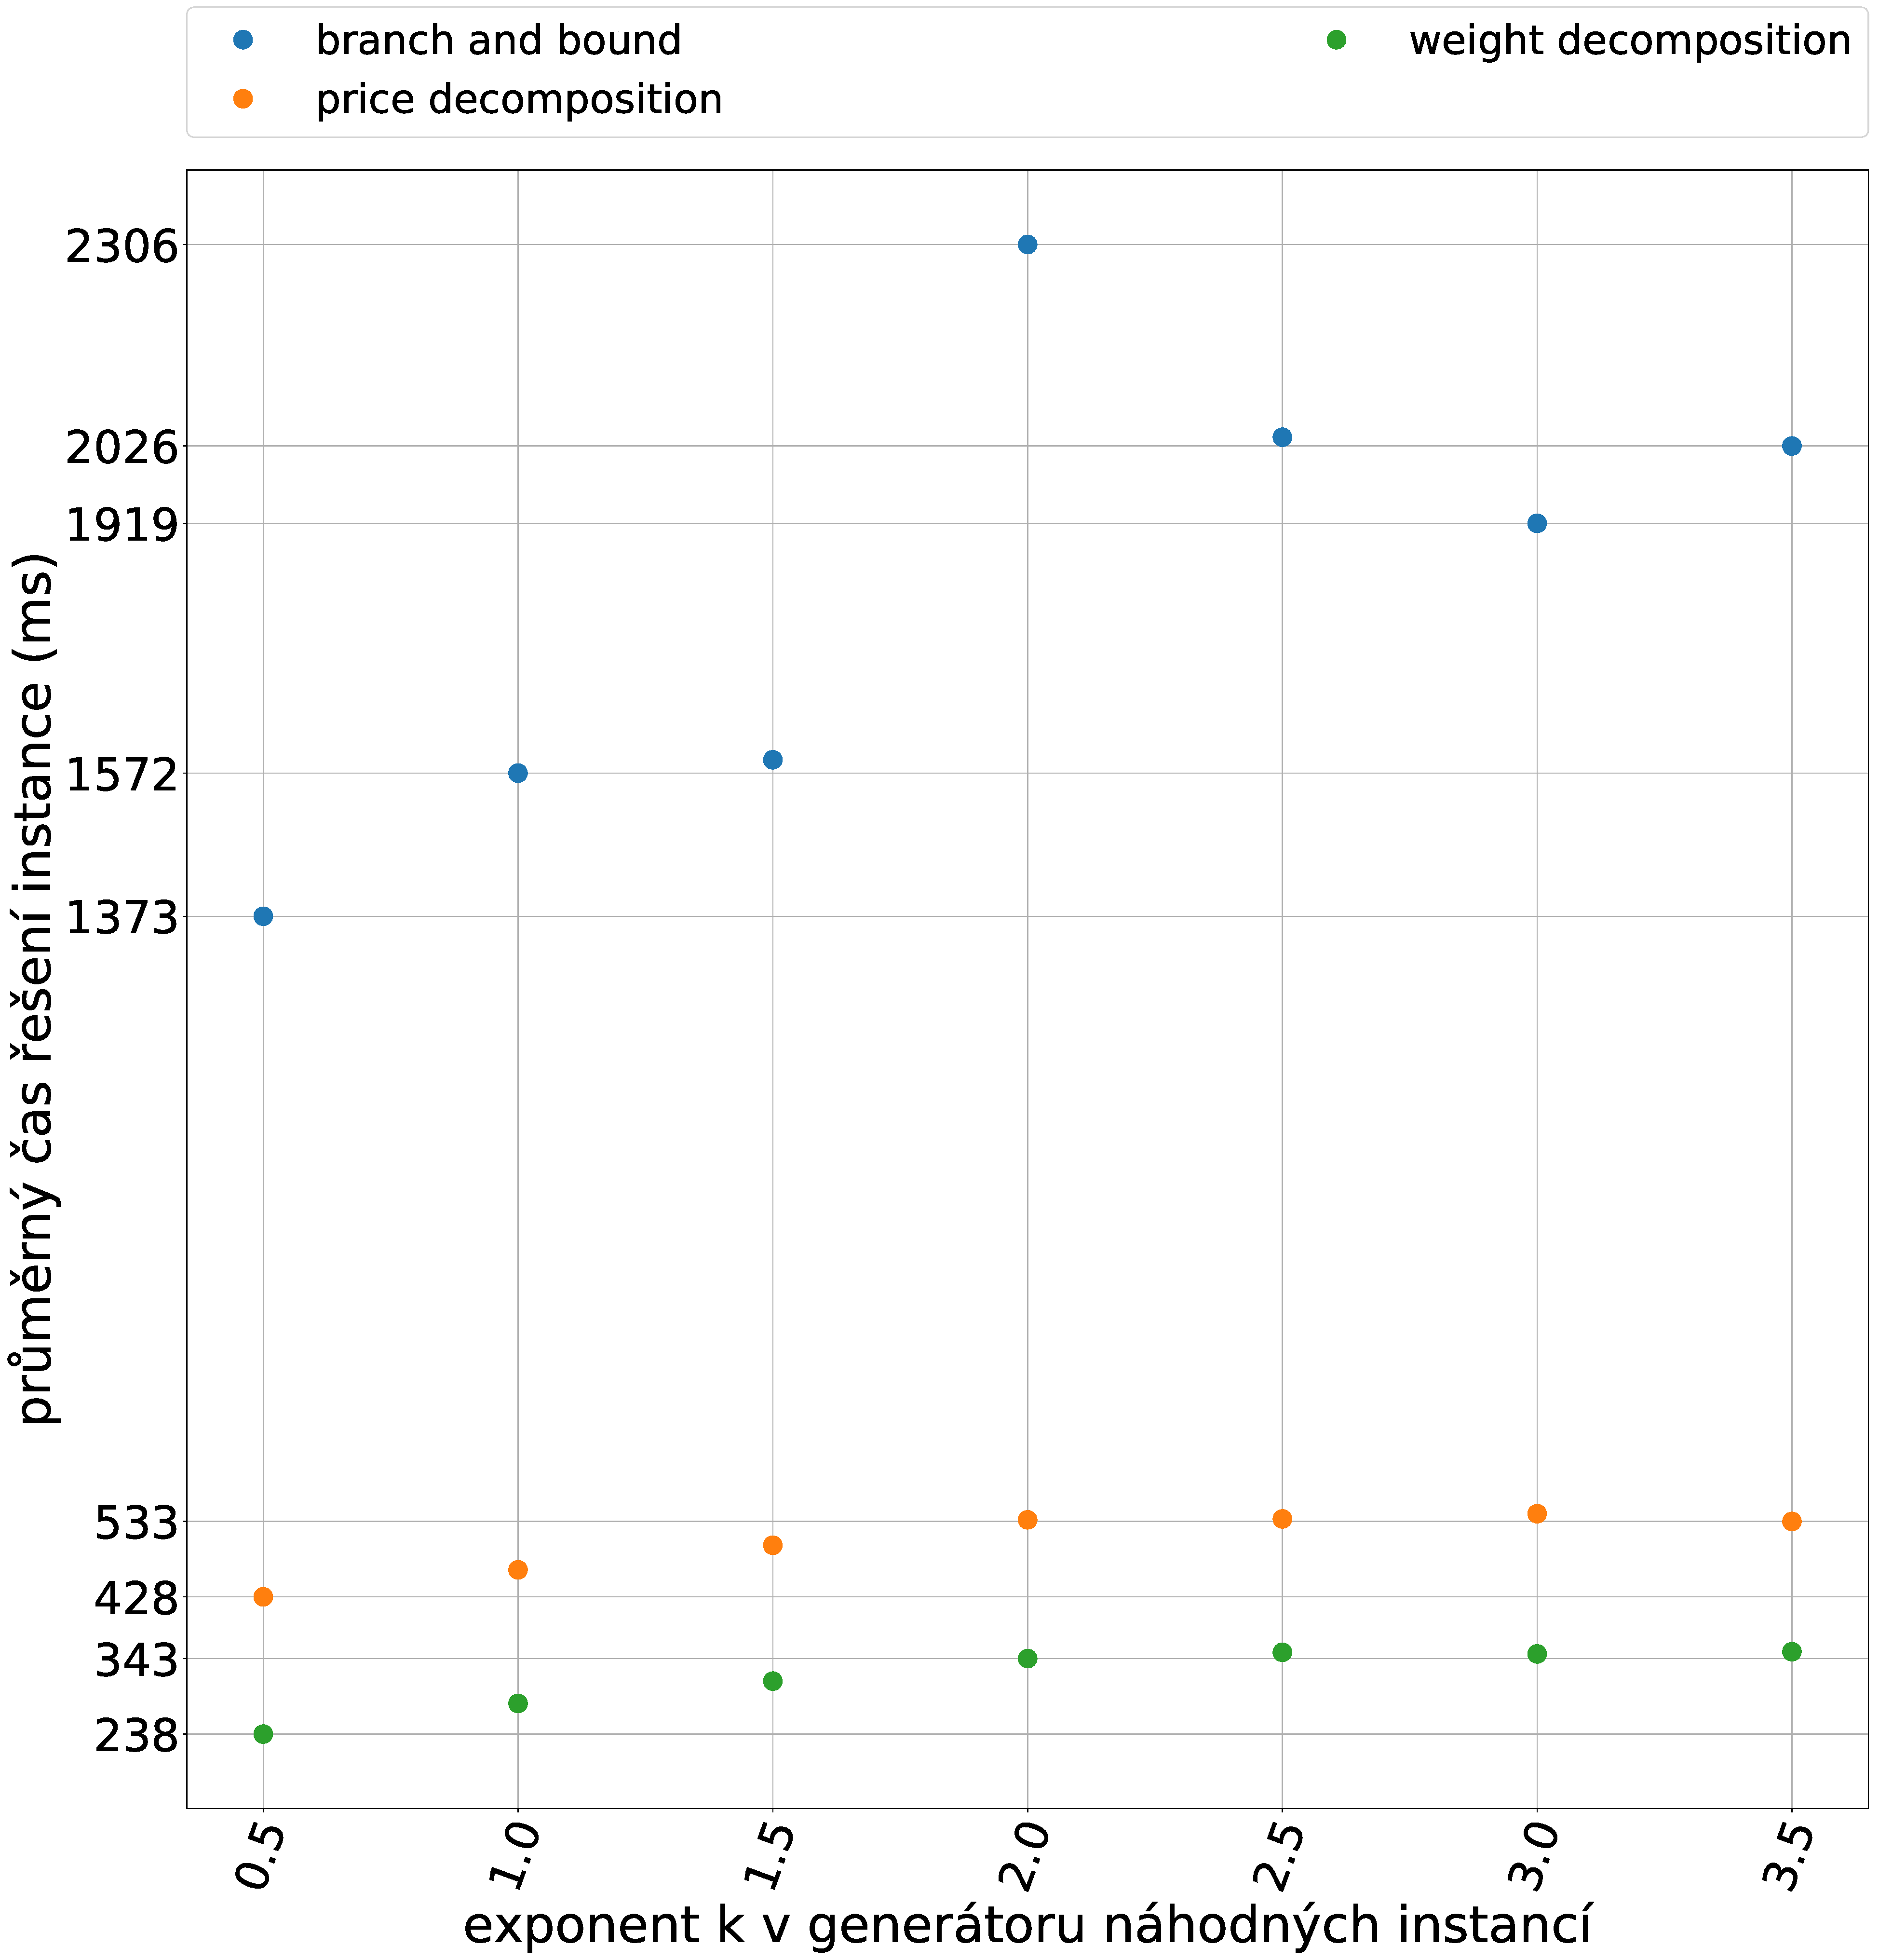
\includegraphics[width=\textwidth]{img/GVE.pdf} 
    \end{minipage}
    \begin{minipage}[c]{0.49\textwidth}
        \centering 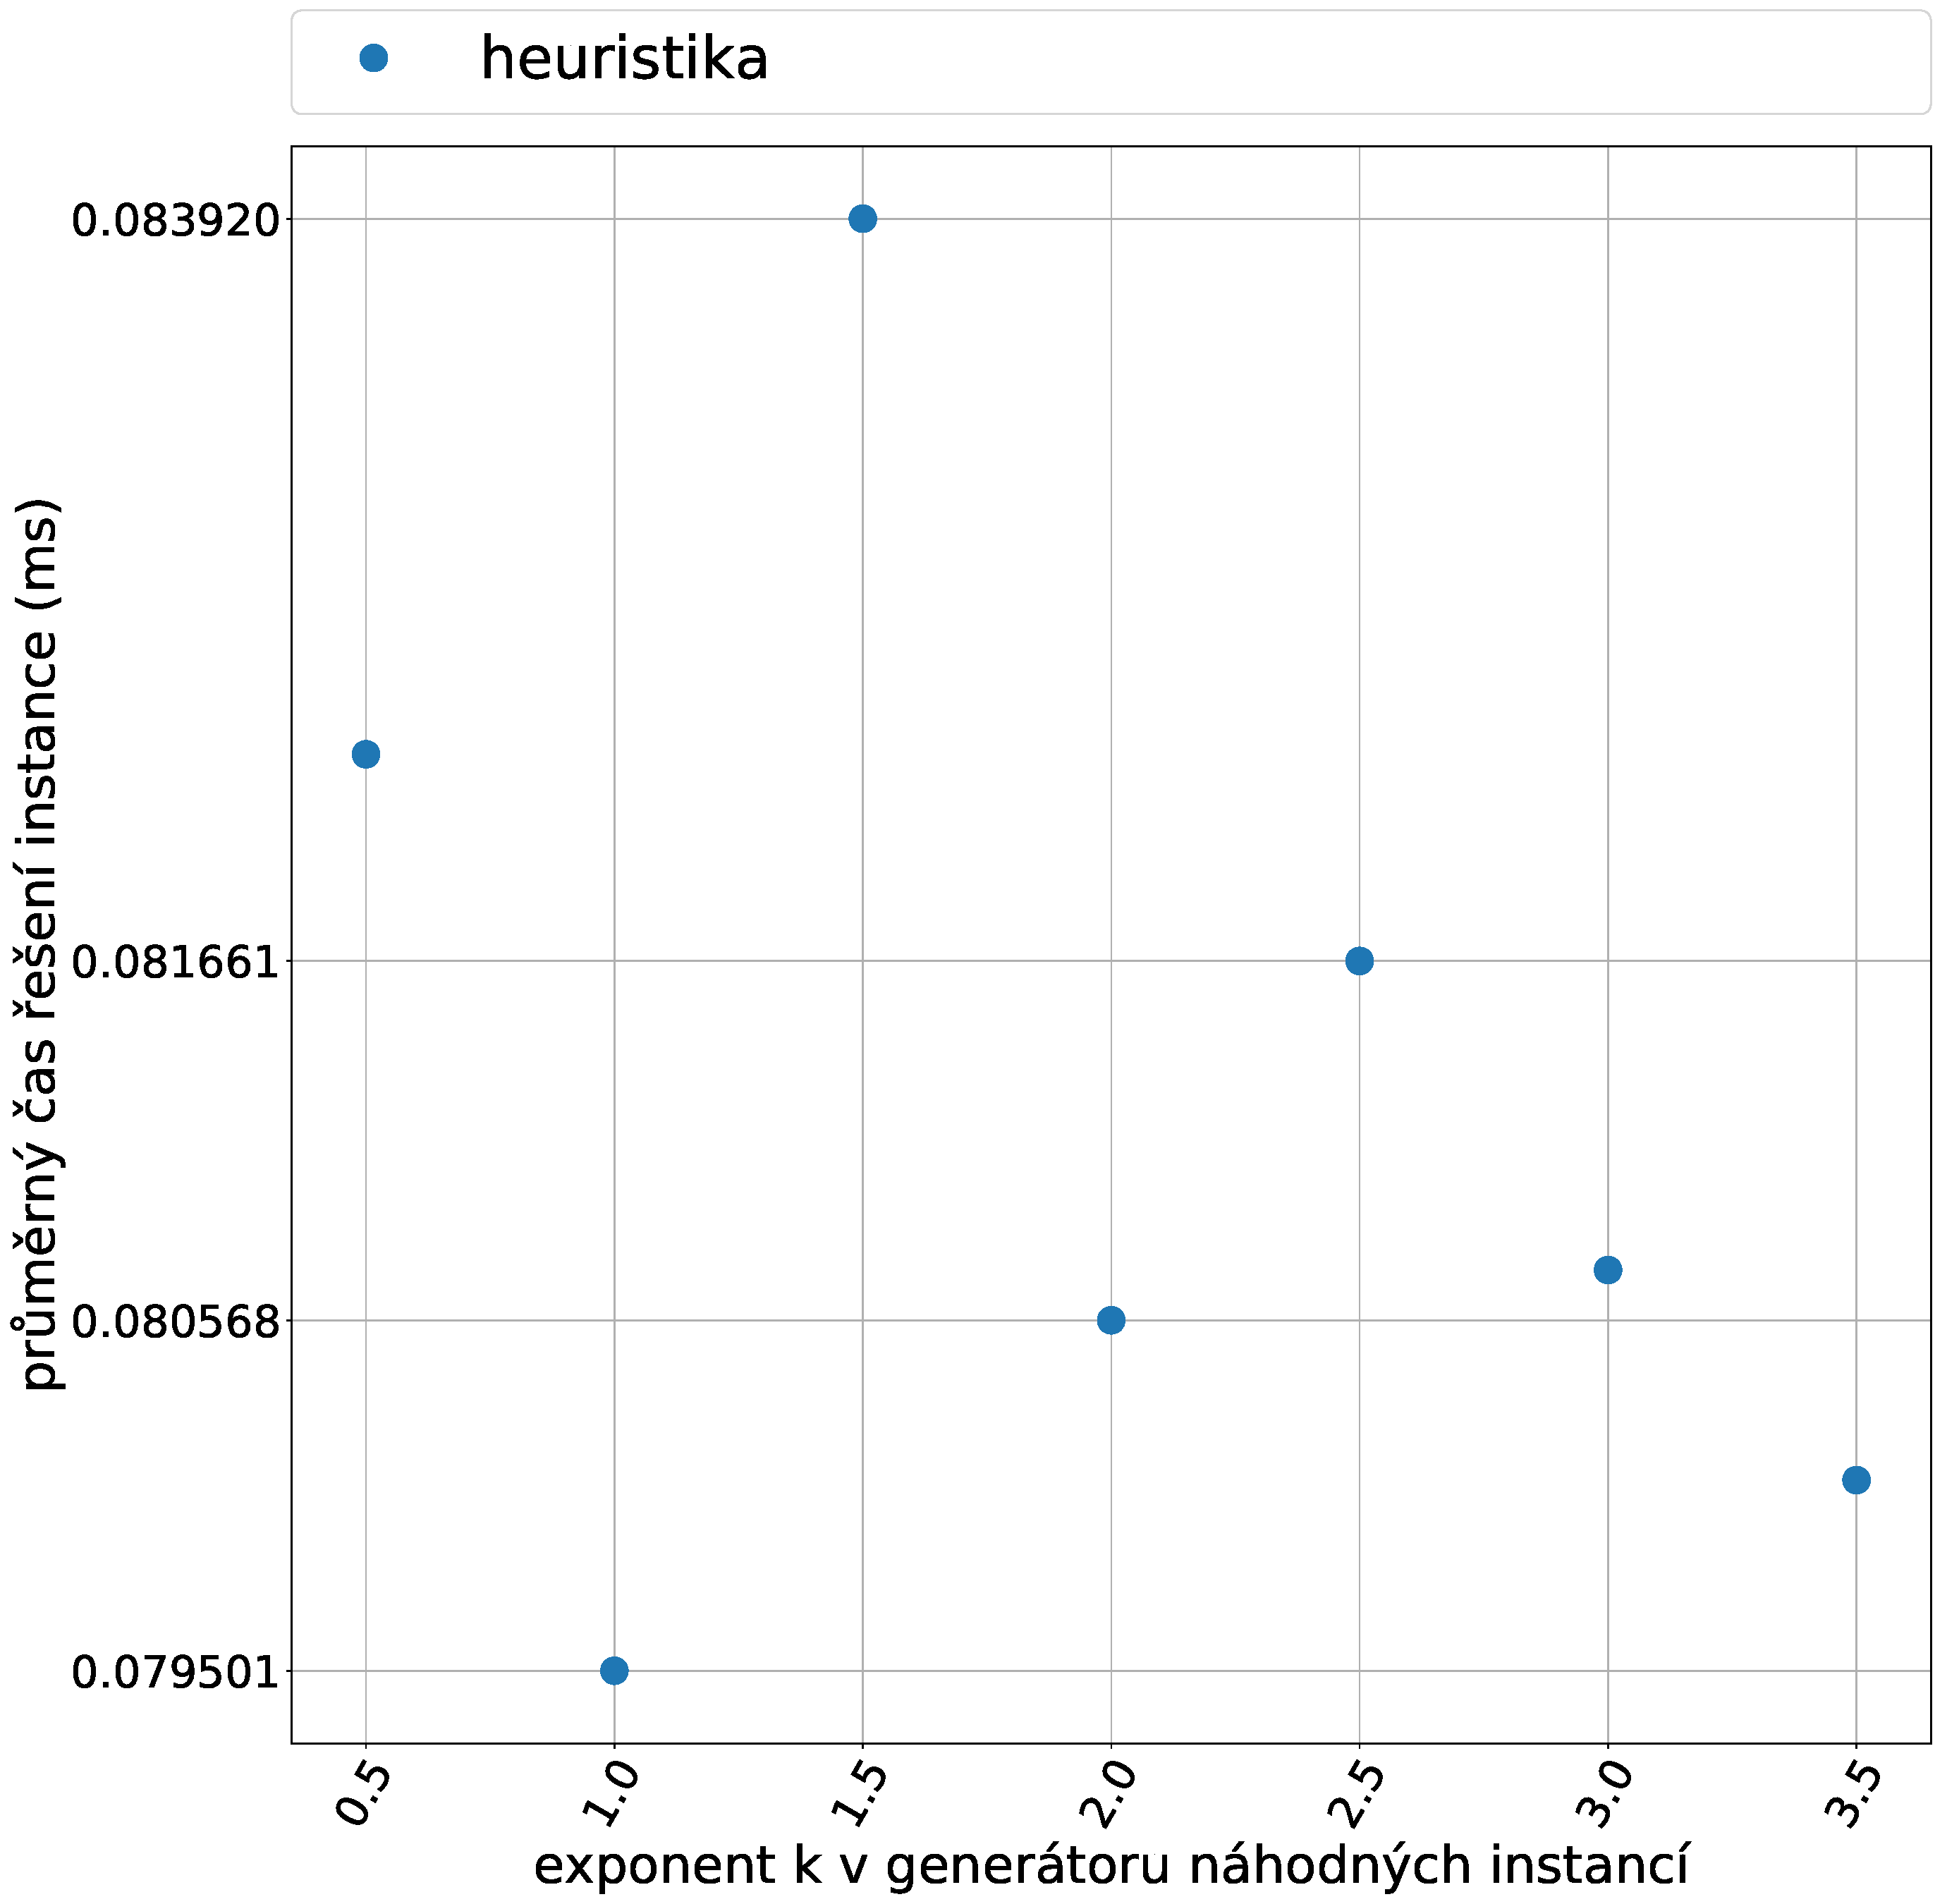
\includegraphics[width=\textwidth]{img/GVH.pdf} 
    \end{minipage}
    \\
   \caption{Na grafech je zobrazena časová náročnost jednotlivých medod v závislosti na granularitě instance. Zde jsou uvedeny grafy pro převahu velkých instancí, kde k je exponent z generátoru náhodných instancích, který určuje pravděpodobnost přijetí daného předmětu.}\label{fig:GVI}
   
    \end{figure} 
    
    \begin{figure}
	\centering
    \begin{minipage}[c]{0.49\textwidth}
        \centering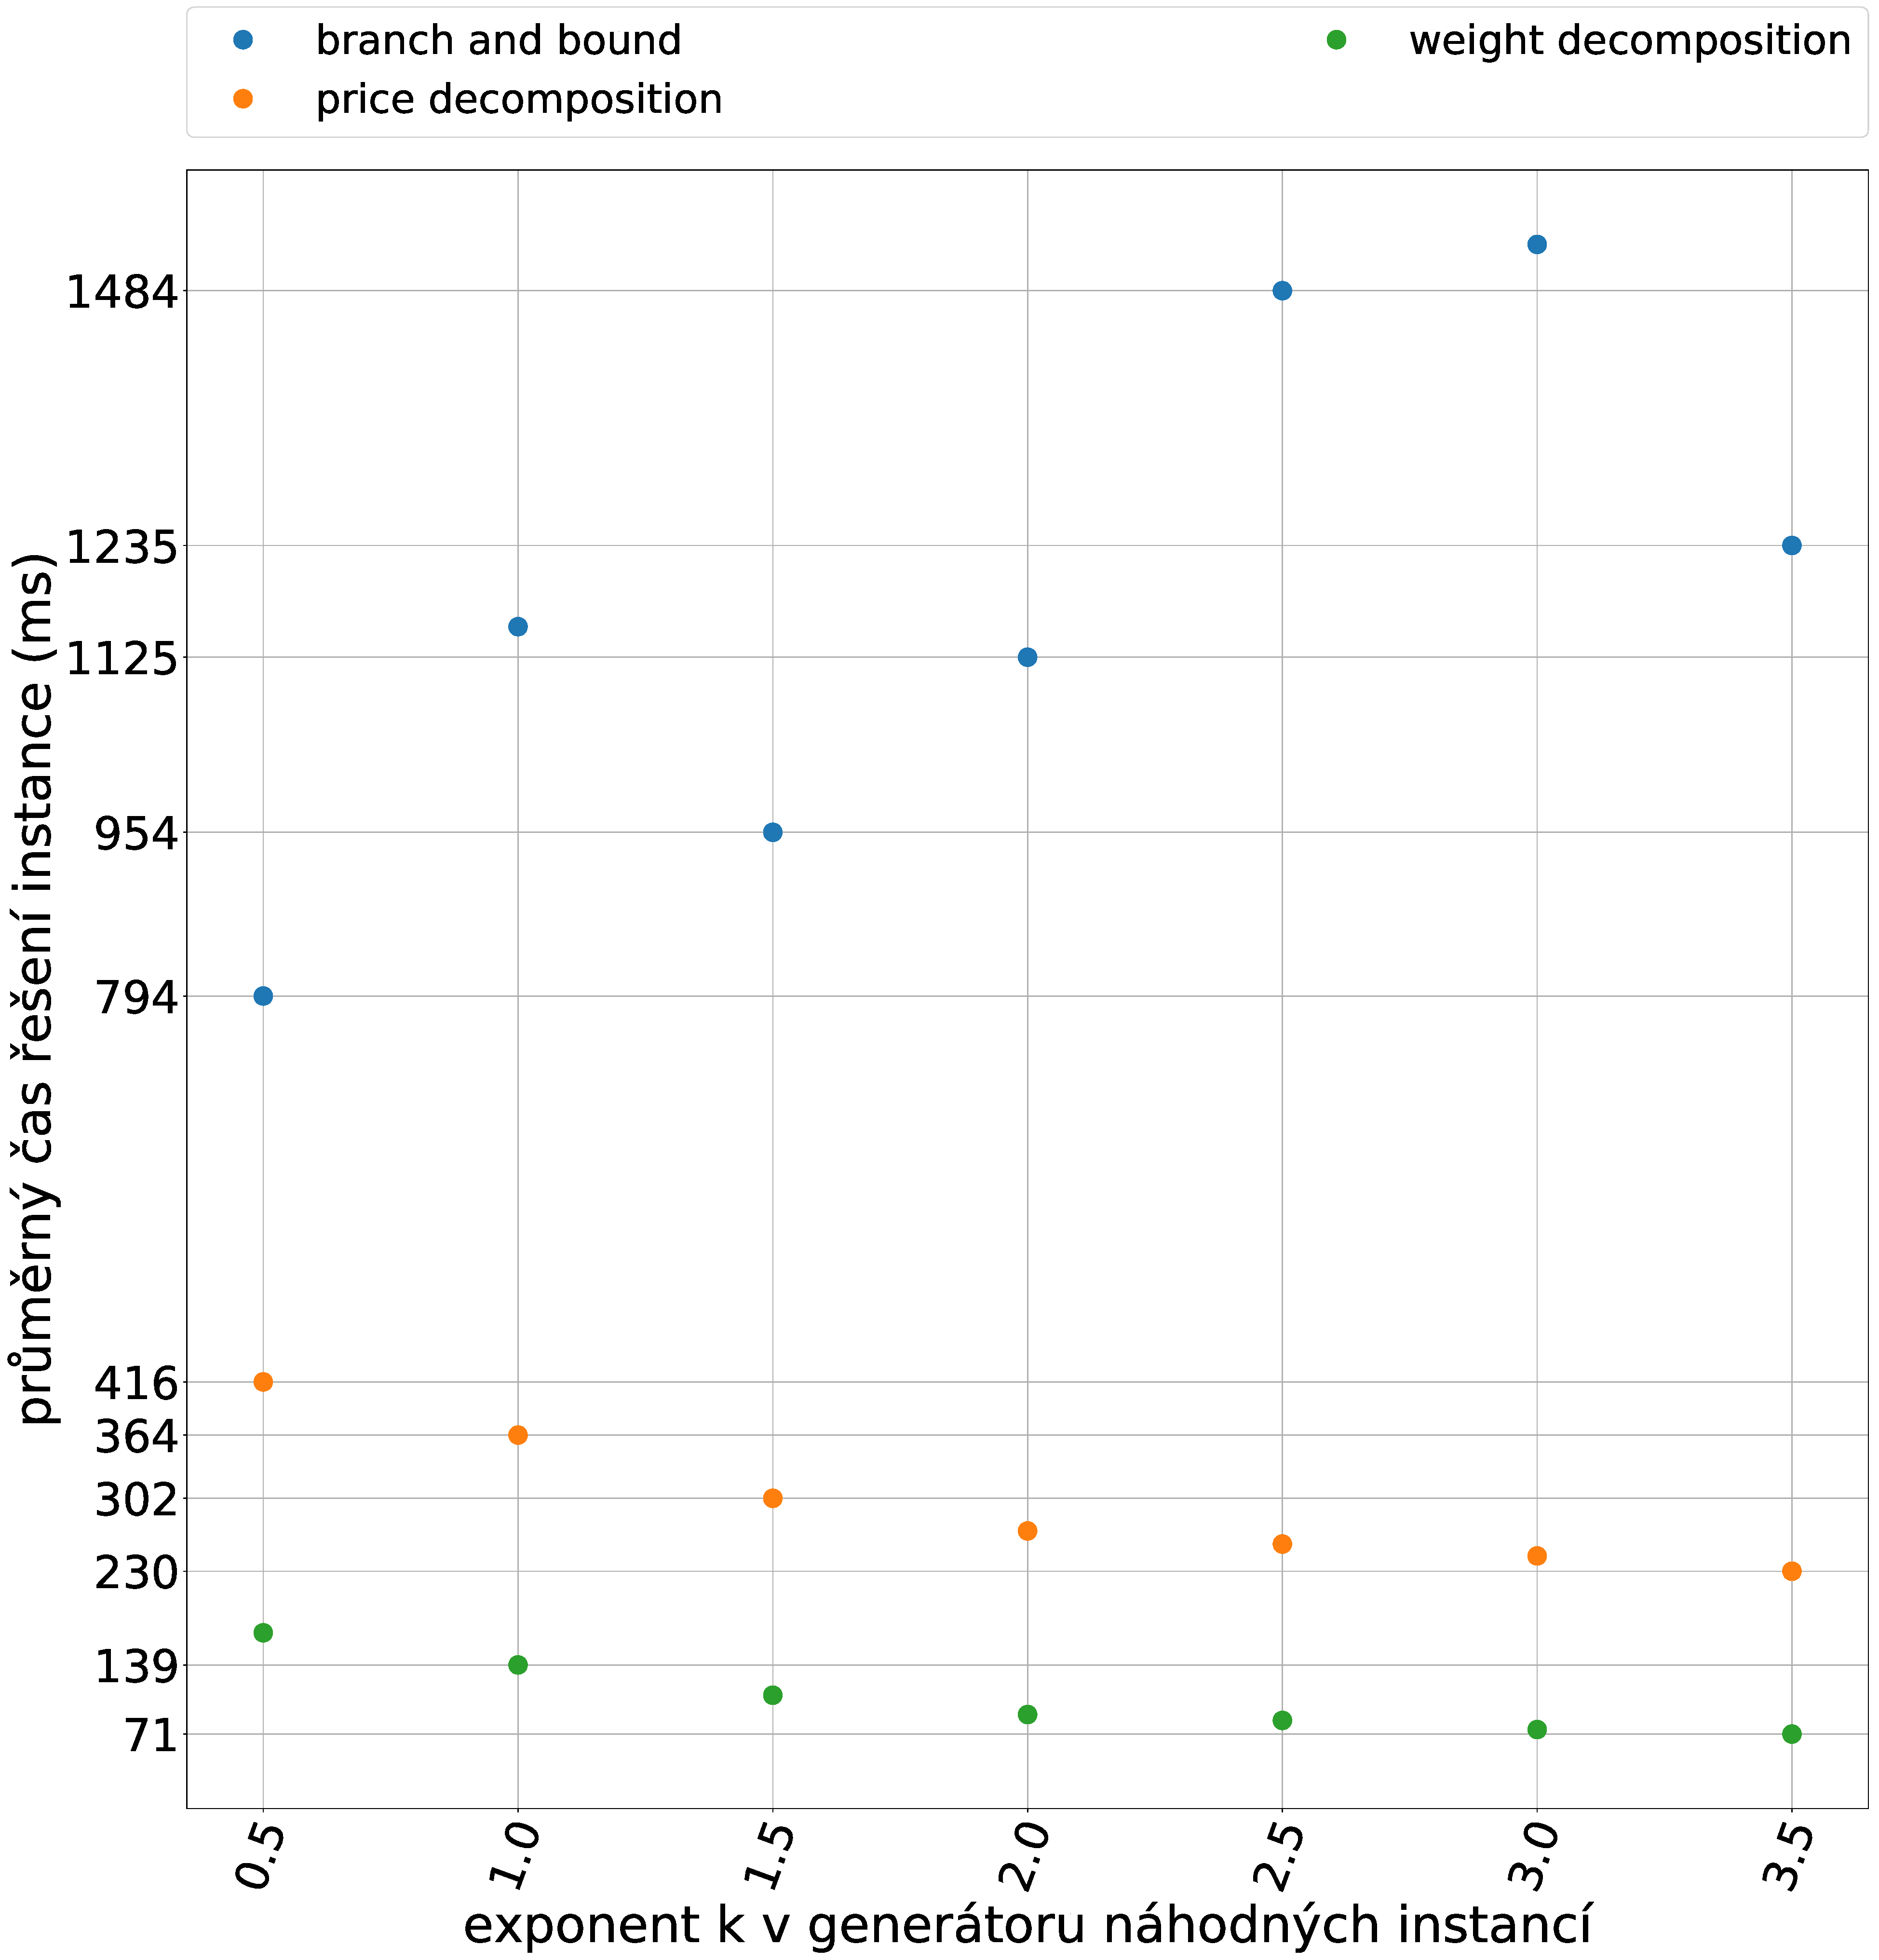
\includegraphics[width=\textwidth]{img/GME.pdf} 
    \end{minipage}
    \begin{minipage}[c]{0.49\textwidth}
        \centering 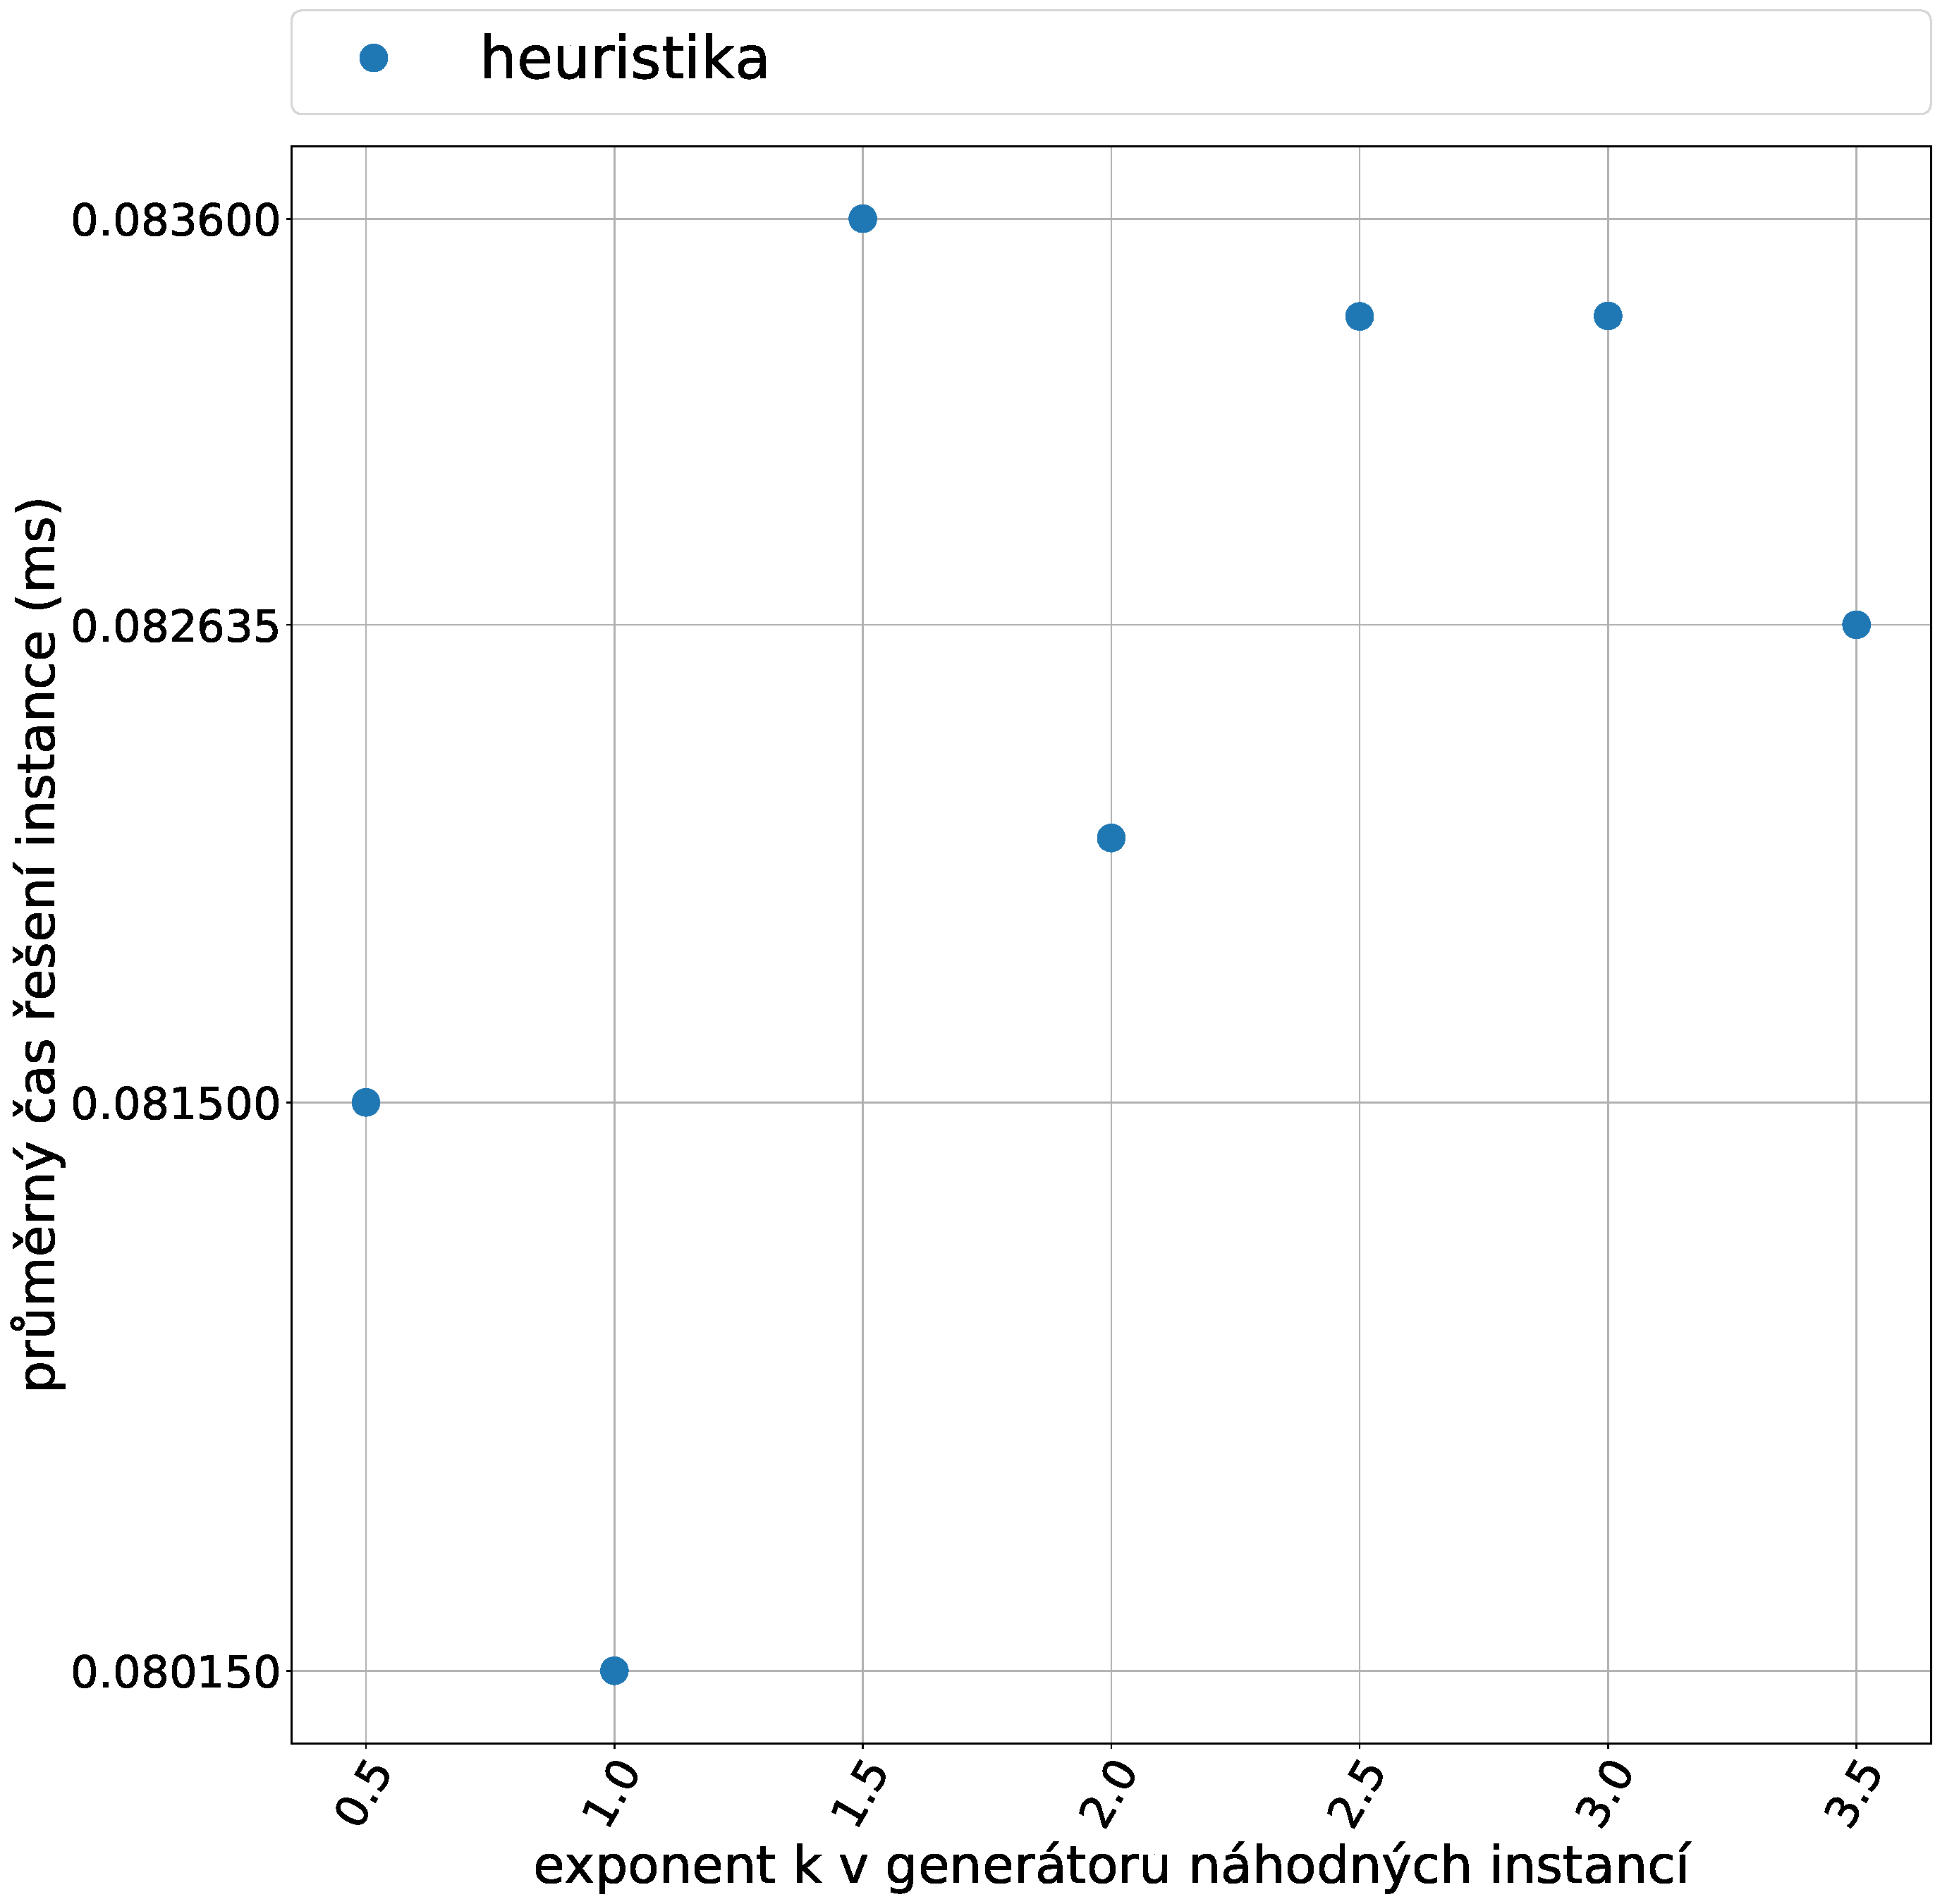
\includegraphics[width=\textwidth]{img/GMH.pdf} 
    \end{minipage}
    \\
   \caption{Na grafech je zobrazena časová náročnost jednotlivých medod v závislosti na granularitě instance. Zde jsou uvedeny grafy pro převahu malých instancí, kde k je exponent z generátoru náhodných instancích, který určuje pravděpodobnost přijetí daného předmětu.}\label{fig:GMI}
    \end{figure} 
 

 
 
Experimenty jsem prováděl v režimu jednoho vlákna na starším datovém serveru v podobě starého notebooku, který v době výpočtu nebyl používán. Výsledky tedy nejsou ovlivněny jinými běžícími programy. Procesor na testovacím stroji: \textit{Intel Pentium T3400 (2 cores). Taktován na 2.16~GHz s~1~MB cache}.
Měření času CPU probíhalo v knihovně $timeit$ s tisíci násobným průchodem pro jednotlivá měření pro přesnost měření.

Pro každý parametr bylo vygenerováno 100 instancí o počtu předmětů 27. Ostatní základní parametry jsem uvedl v tabulce \ref{tab:GVI}. Při jednotlivých experimentech byl vždycky měněn jeden parametr. Na grafech jsem vždy rozdělil exaktní metody a heuristiku z důvodu nízkých časů u heuristiky, u které by nebyly rozdíly s exaktními metodami vůbec ukázatelné. 

\begin{table}[h]
\centering
    \begin{tabular}{ |l|l| } 
        \hline
        Parametr & Hodnota \\
        \hline
        \hline
        Poměr kapacity batohu k sumární váze & $0.5$ \\
        Maximální váha věci & $50$ \\
        Maximální cena věci & $50$ \\
        Exponent $k$ & $1$ \\
        Velké nebo malé věci v batohu & $0$ \\
        \hline
    \end{tabular}
    \caption{Tabulka základního nastavení parametrů generátoru.}\label{tab:GVI}
\end{table} 
 


\subsection{Závislost na granularitě instance}
První jsem se podíval na granularitu instancí. Ta je řízena následovně. V generátoru je možno ovlivnit, zda instance bude obsahovat spíše malé nebo spíše velké věci. Pro převahu malých věcí je pravděpodobnost $p$, že věc s váhou $w$ bude v instanci zahrnuta $$ p=\frac{1 }{ w^k}$$. Kde $k$ je volitelný exponent. Pro převahu velkých věcí platí symetrický vztah $$ p=\frac{1}  {(w_{max}-w)^k}$$.

Na grafu \ref{fig:GVI} můžeme vidět porovnání pro převahu velkých věcí. Lze vidět, že pro metody větví a hranic je zde jasně patrný trend. S větším počtem velkých předmětů tedy roste její výpočetní náročnost. Tento trend, avšak ne tak patný, může být pozorován i na jednotlivých dekompozicích. 

Na grafu \ref{fig:GMI} vidíme porovnání pro převahu malých věcí. I zde jsou patrné citlivosti jednotlivých exaktních metod. Ale mírně odlišně než u převahy velkých věcí. U metody větví a hranic je stále s převahou menších instancí roste její časová náročnost. Naopak u dekompozicích tento čas klesá. 

Citlivost u dekompozic bych si také mohl vysvětlit jako citlivost na celkovou sumu váhy nebo ceny podle druhu dekompozice. Protože převaha velkých nebo malých předmětů tuto sumu ovlivní. Citlivost na tyto parametry prozkoumáme v další podkapitole.

U heuristické metody na grafech můžeme vidět veliký rozptyl hodnot. Její závislost na granularitě se tady nepotvrdila. O této metodě bych tedy neřekl, že její výkonost ovlivní granularita jednotlivých instancí.

Na grafech \ref{fig:GOEI} je ukázána průměrná a maximální chyba heuristické metody při změnách granularity instancí. Zde není patrná témě žádná závislost chyby na granularitě instance. Při podrobnější zkoumální hodnot maxim, by možná bylo možné říct, že maximální chyba klesá s převahou malých i velkých předmětů, ale tento trend by bylo nutné podrobněji prozkoumat a podrobit mnohem větší analýze.
 
 \begin{figure}
	\centering
    \begin{minipage}[c]{0.49\textwidth}
        \centering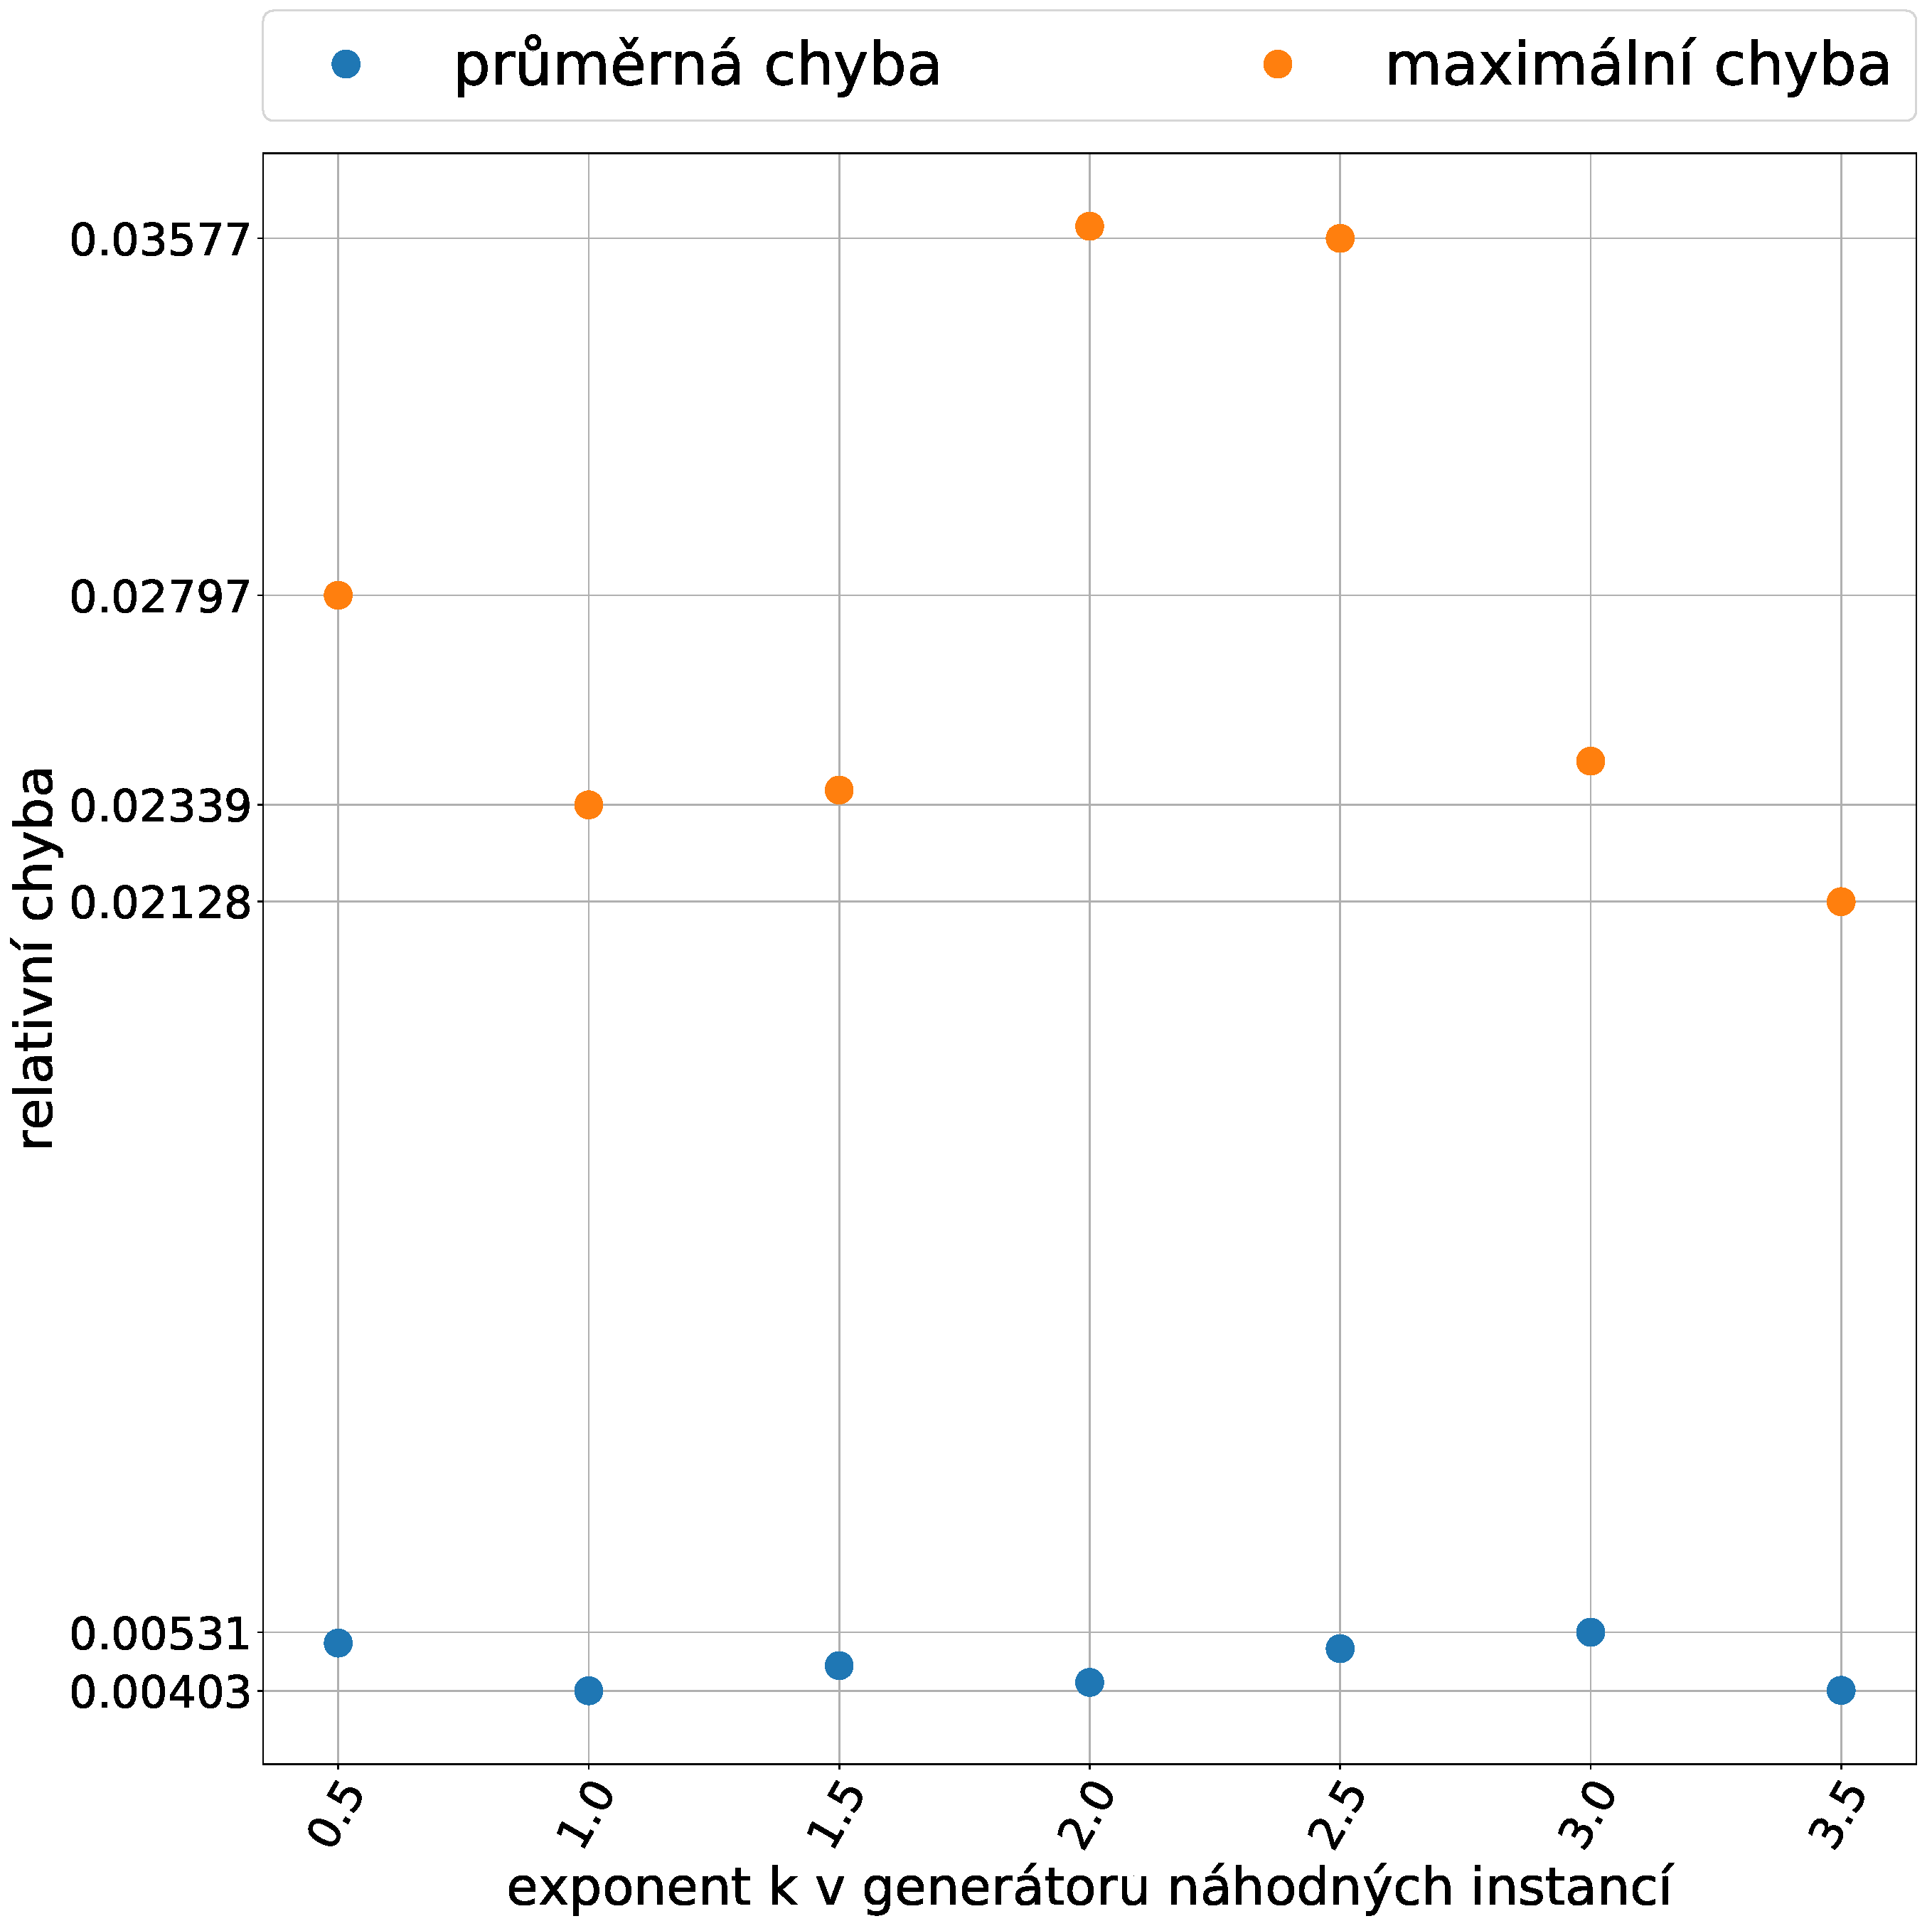
\includegraphics[width=\textwidth]{img/GMHE.pdf} 
    \end{minipage}
    \begin{minipage}[c]{0.49\textwidth}
        \centering 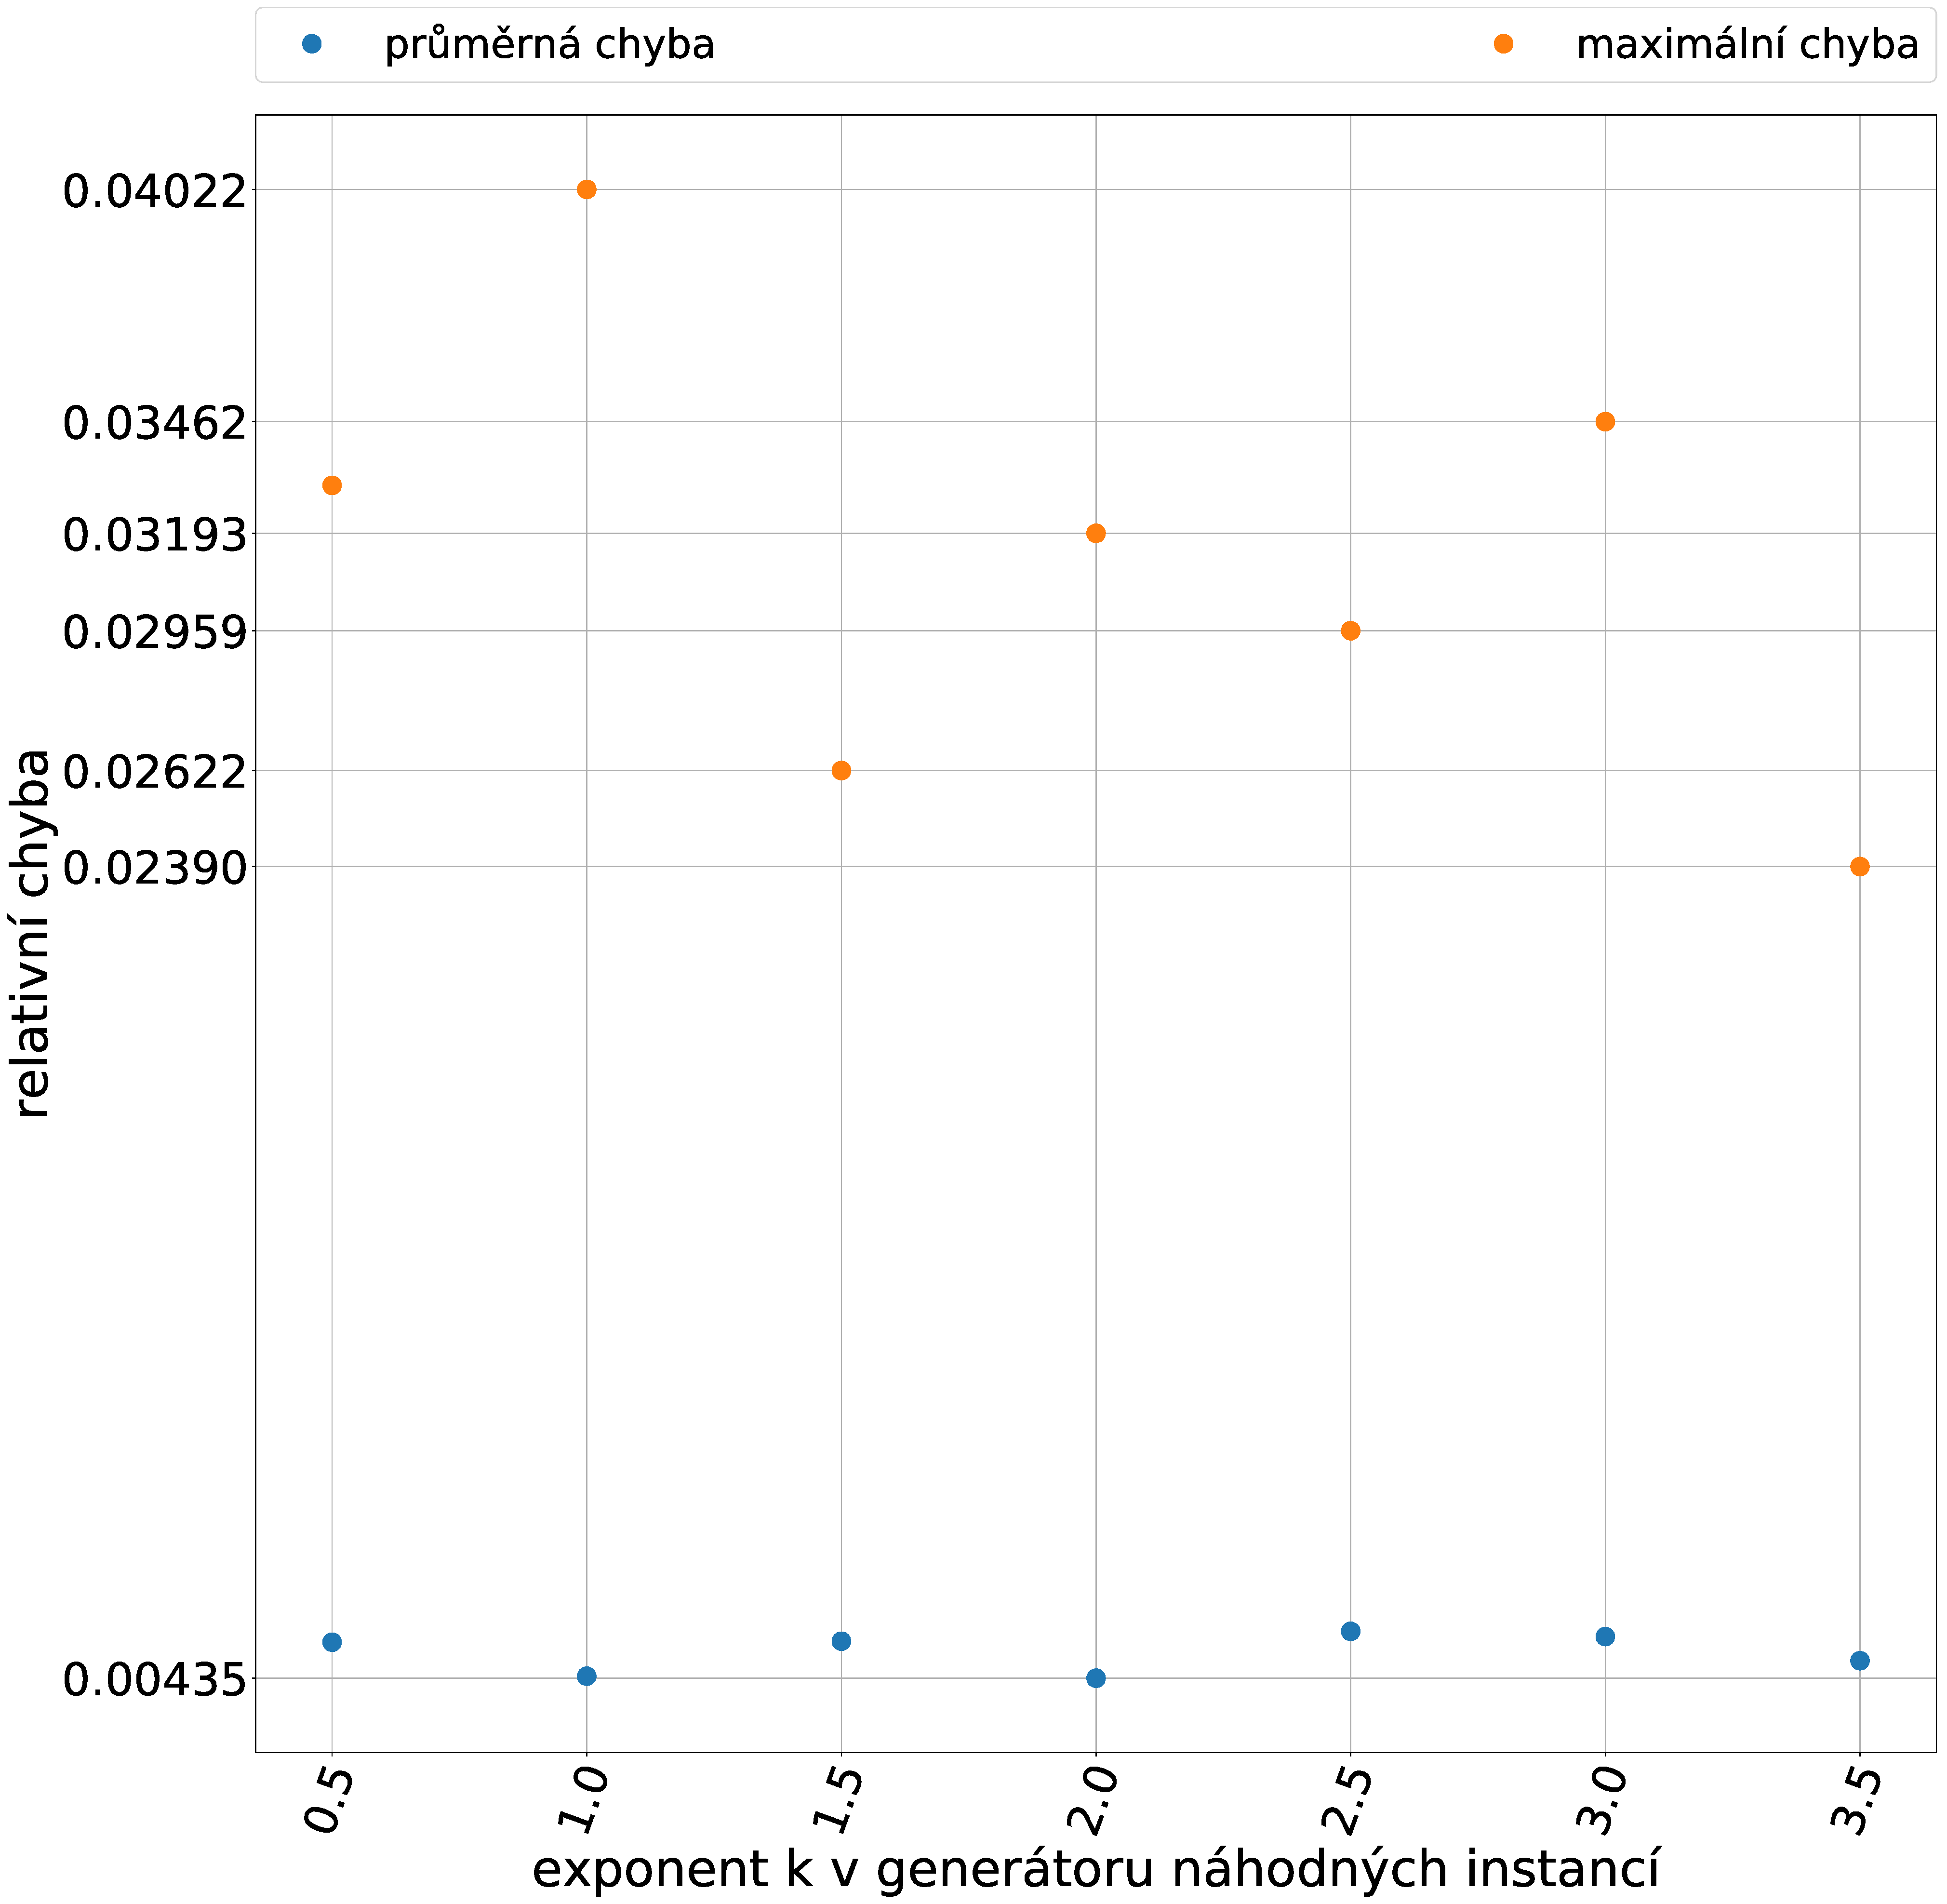
\includegraphics[width=\textwidth]{img/GVHE.pdf} 
    \end{minipage}
    \\
   \caption{Na grafech je ukázána vždy průměrná a maximální chyba heuristiky v závislosti na granularitě instance. Na levém grafu pro převahu malých instancí a na převém grafu pro převahu velkých instancí.}\label{fig:GOEI}
    \end{figure} 
    
\subsection{Závislost na poměru součtu vah předmětů k nosnosti batohu}
Pro tento parametr jsem očekával největší citlivost u metody větví a hranic. Tato citlivost se potvrdila a je patná na grafu \ref{fig:mI}. Je tedy zjevné, že metoda selhává v momentě, kdy se optimální řešení skládá z většího počtu předmětů. Také je na grafu vidět pád pro hodnotu 1. Tento jev je očekávaný z implementace. V rekurzivním volání se snažím předmět přidávat dokud nedojde k prořezu a v tomto případě končí po přidání všech předmětů.

Pro dynamické programování se výpočetní náročnost také zvyšuje. Toto může být způsobeno tím, že přestává být tak učínné prořezání a je nutné projít více větví rekurze.

Pro heuristiku je také patrný trend, že výpočetní čas roste s poměrem, ale v tomto případě nejsou rozdíly v náročnosti tak velké.

Pro chybu na grafu \ref{fig:mEI} je jasně patrný klesající trend, tedy že chyba je závislá na poměru sumární váhy ke kapacitě batohu. Čím výšší je poměr, tím menší je chyba, protože klesá i pravděpodobnost toho, že předmět nebude v řešení. Nulová chyba pro poměr 1 je očekávána, neboť jsou přídány všechny předmětu do batohu.

\begin{figure}
	\centering
    \begin{minipage}[c]{0.49\textwidth}
        \centering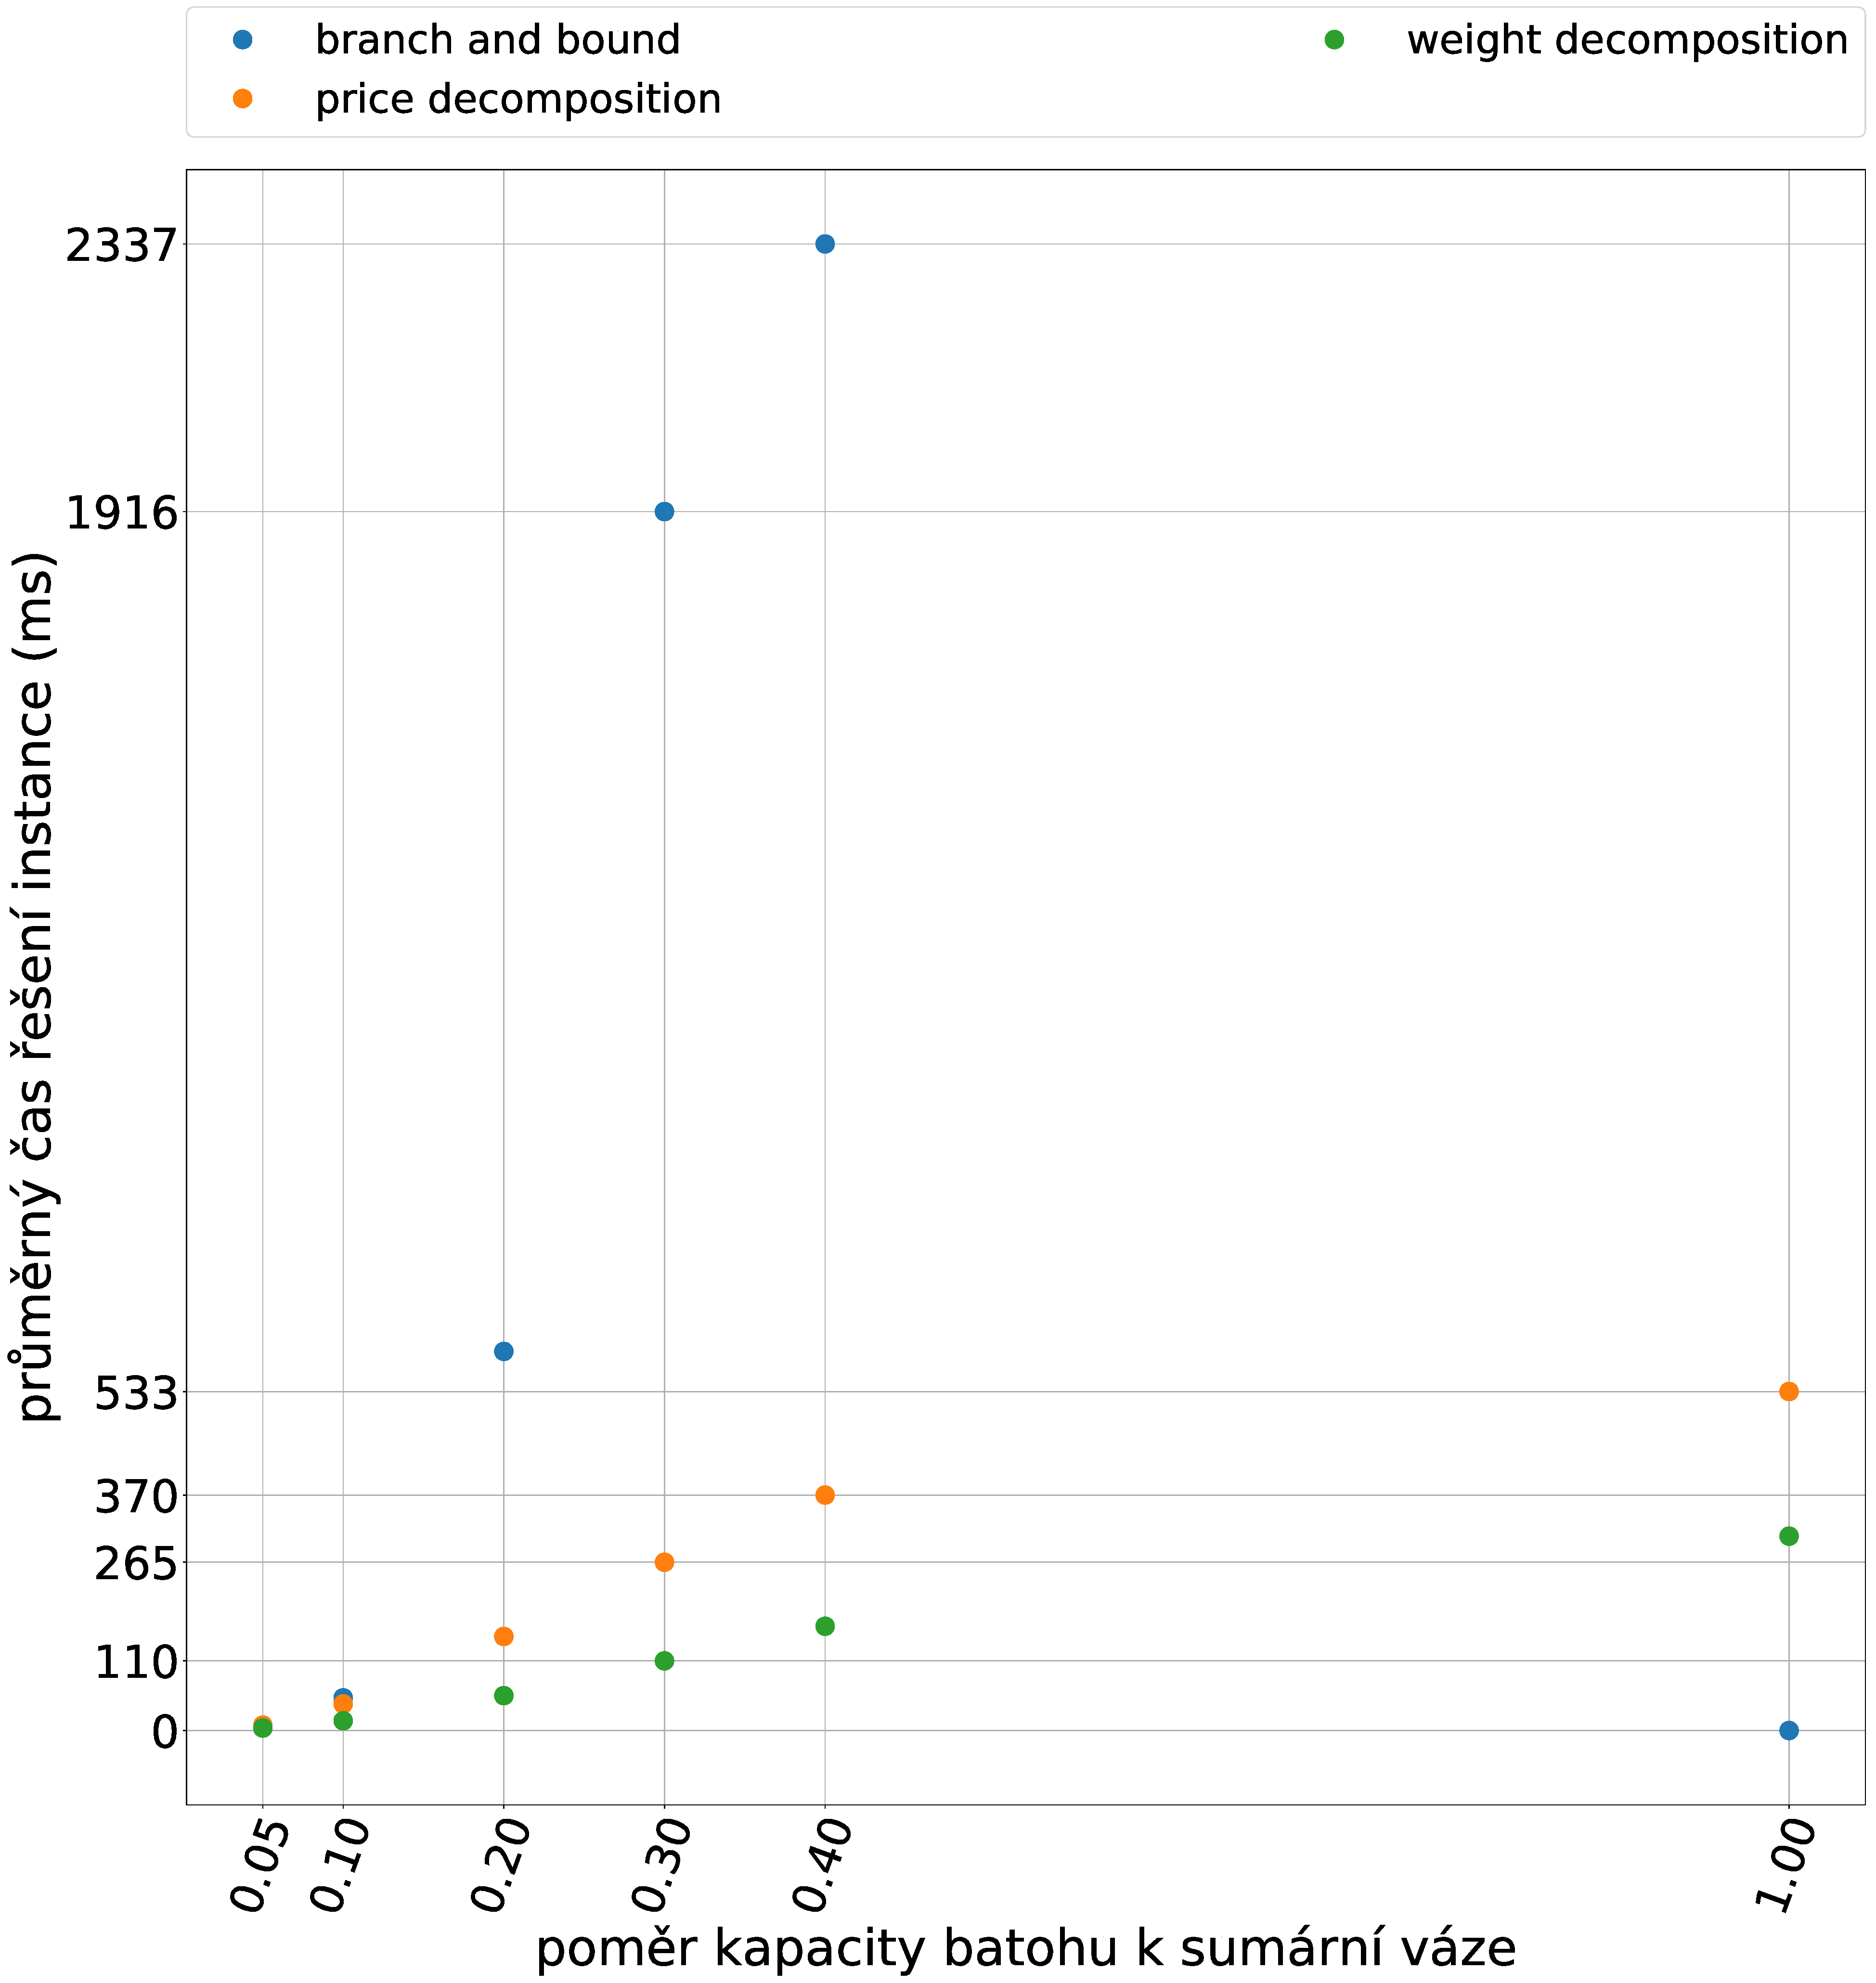
\includegraphics[width=\textwidth]{img/mE.pdf} 
    \end{minipage}
    \begin{minipage}[c]{0.49\textwidth}
        \centering 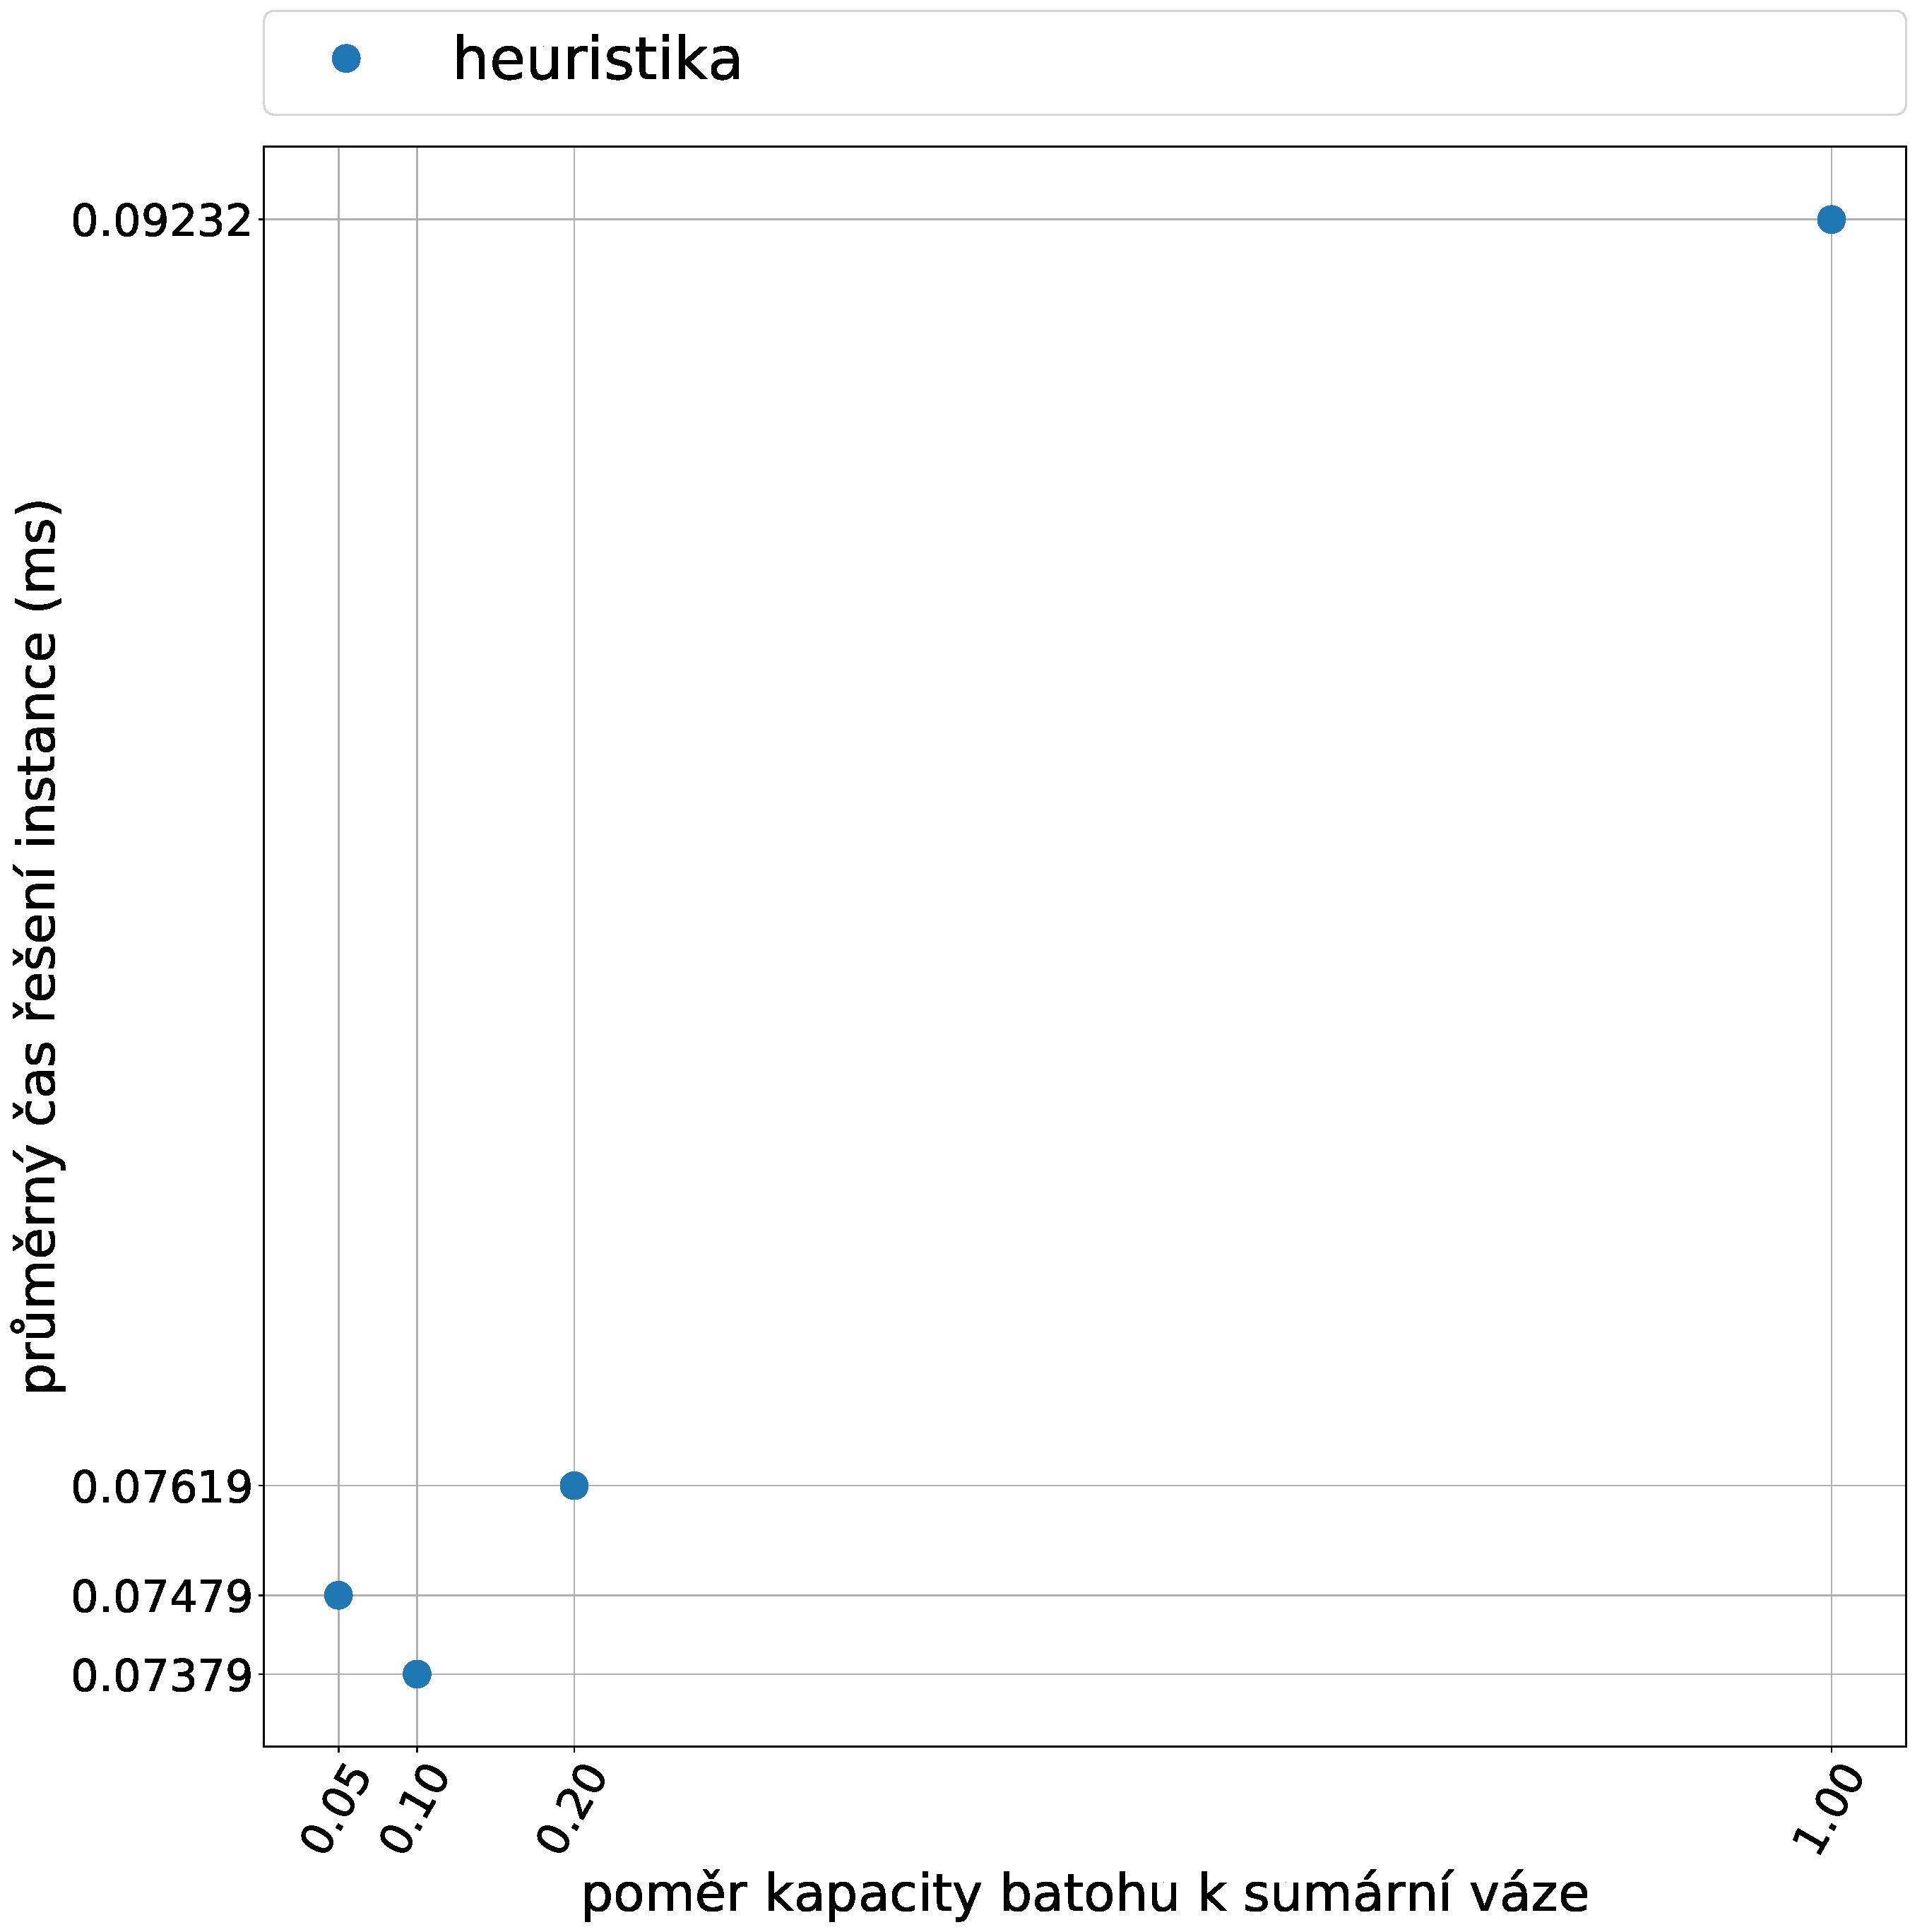
\includegraphics[width=\textwidth]{img/mH.pdf} 
    \end{minipage}
    \\
   \caption{Na grafech je vidět závislost výpočetní náročnosti na poměru součtu vah a nosnosti batohu. Vlevo pro exaktní metody a vpravo pro heuristiku.}\label{fig:mI}
    \end{figure} 
    
    

\begin{figure}\centering
	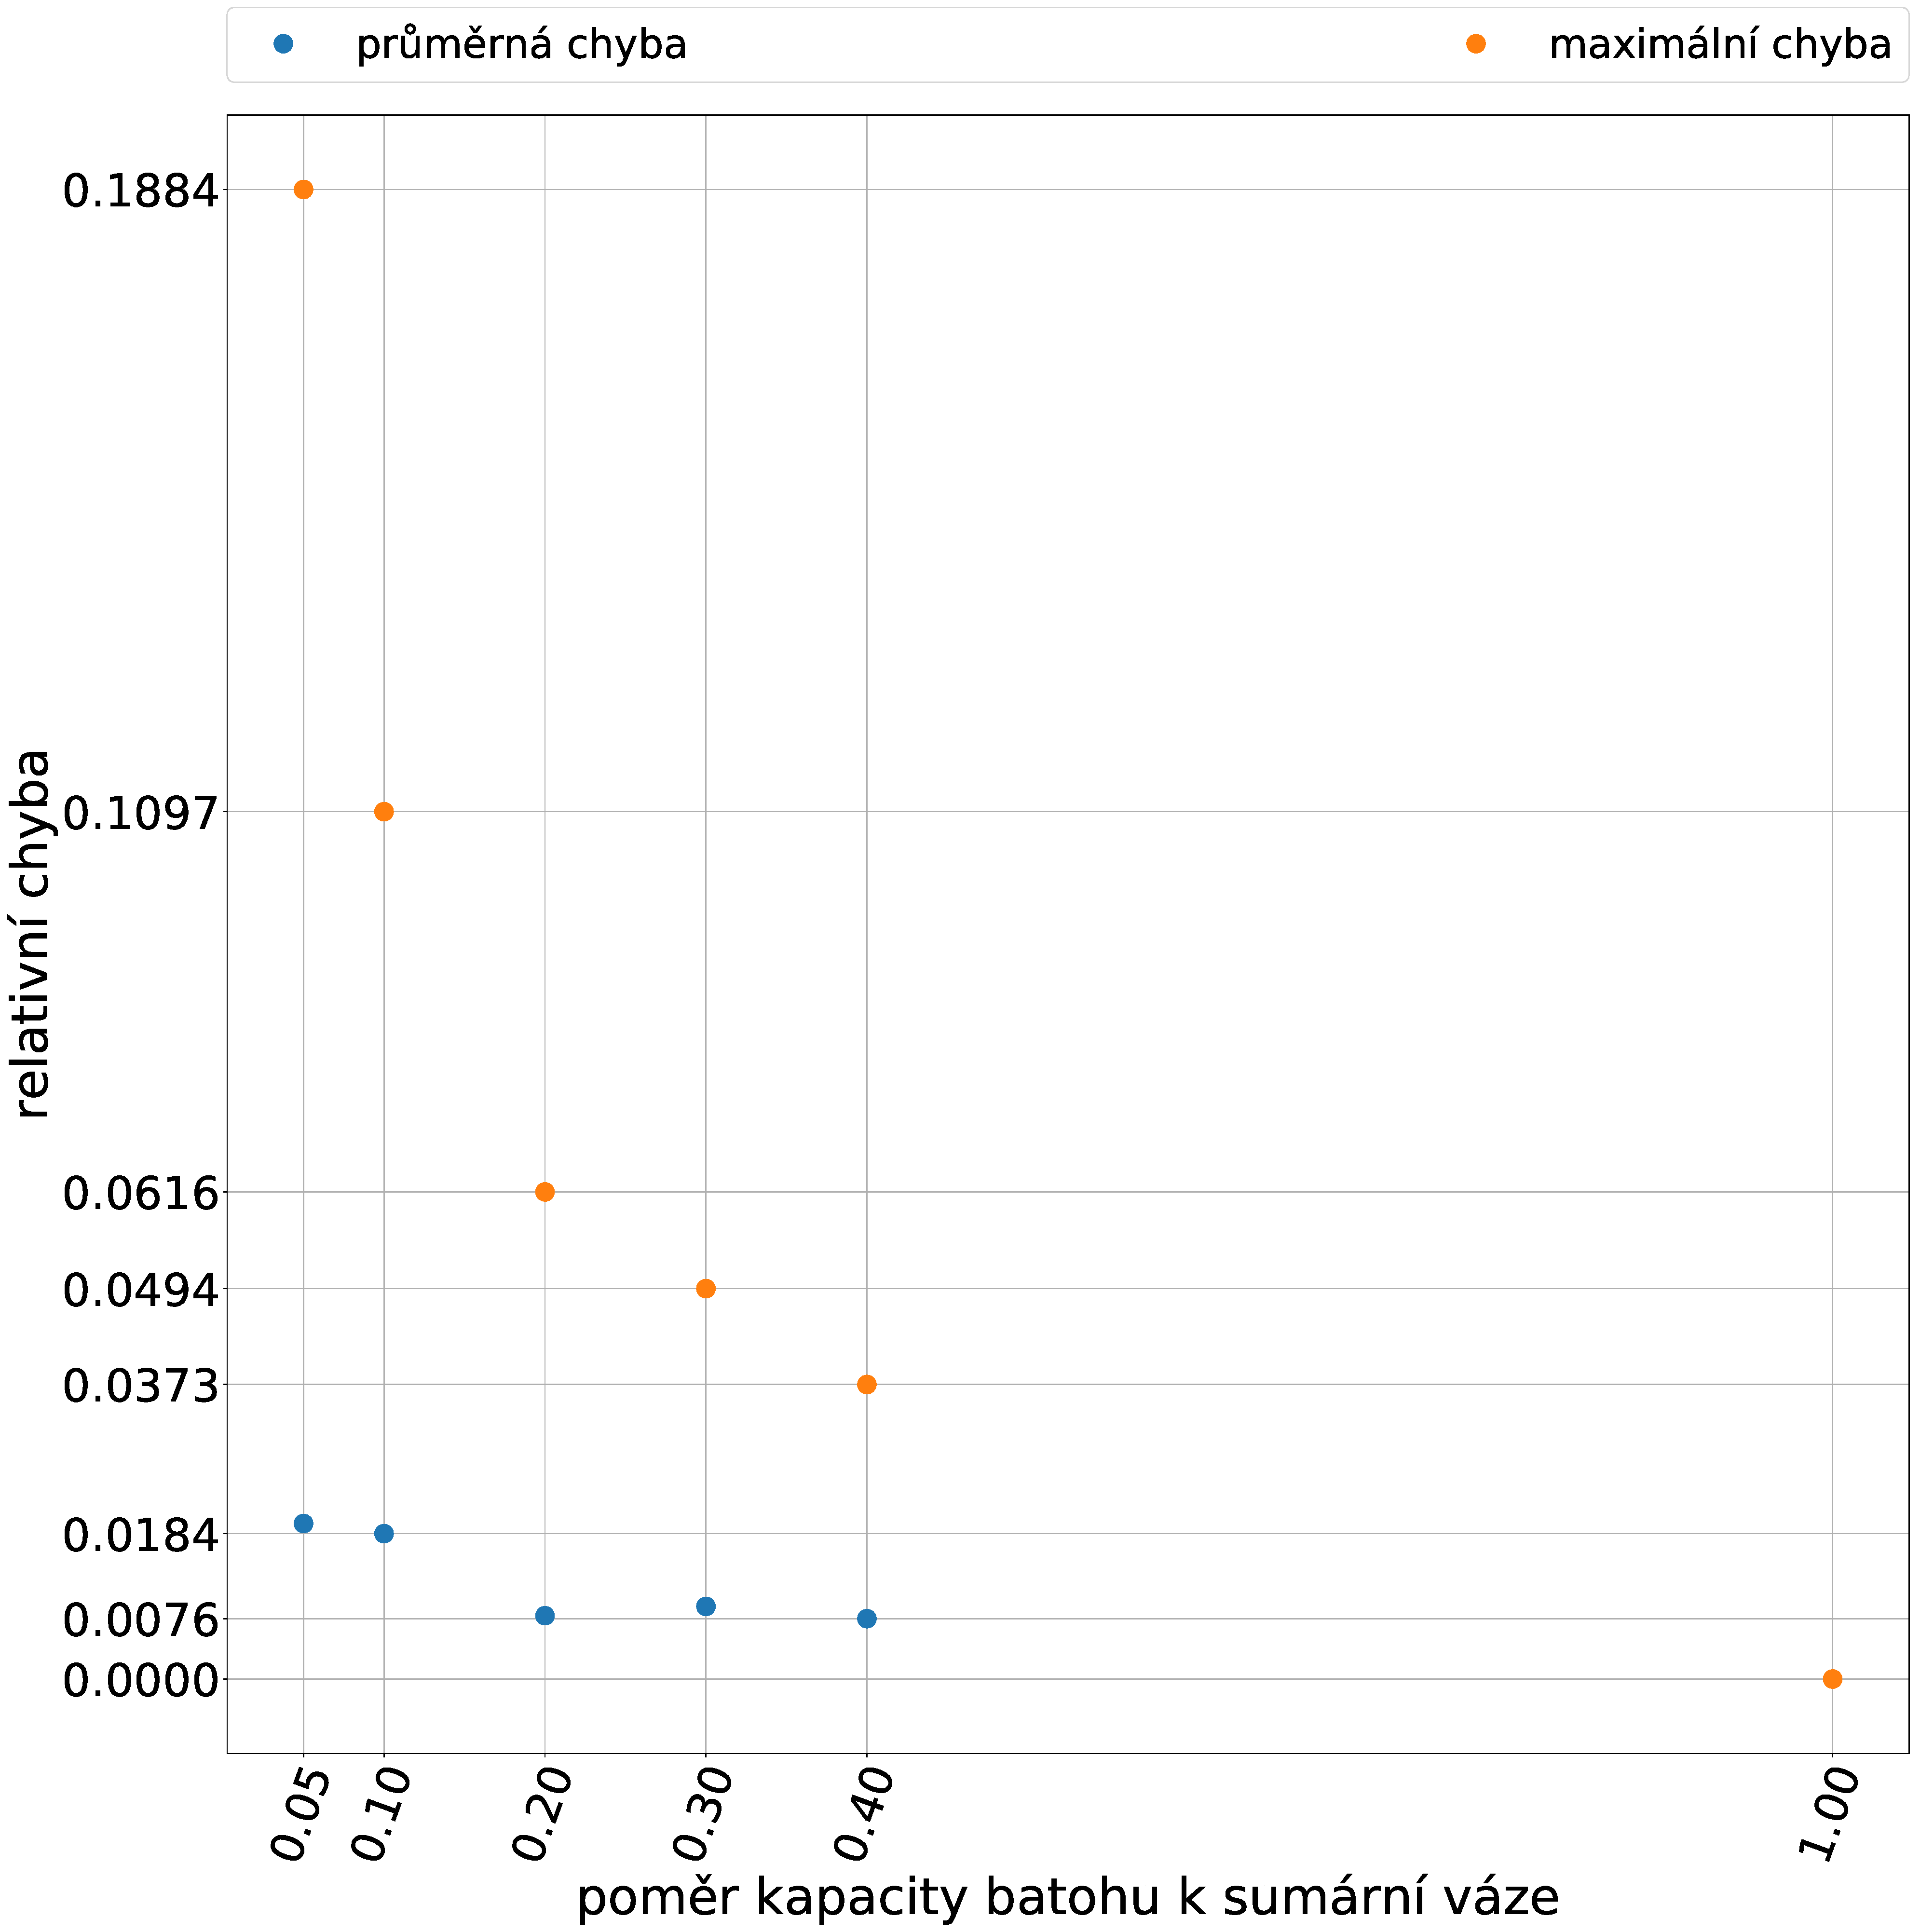
\includegraphics[scale=0.14]{img/mHE}
 	\caption[1]{Relativní chyba heuristiky v závislosti na poměru součtu vah a nosnosti batohu.}\label{fig:mEI}
 \end{figure} 	

\subsection{Závislost na maximální ceně předmětů}

Z grafu \ref{fig:WI} je vidět závislost výpočetní náročnosti na maximální ceně věcí. Zde je opět vidět očekáváný nárůst složitosti u dekompozice podle ceny. Výpočetní náročnost je závislá na tomto parametru, z důvodu akolování prostředků pro tabulku dynamického programování. Tabulka má rozměr v závislosti na součtu vah všech předmětů a počtu předmětů.

Na grafu heuristiky je patrný trend, ale ve velmi malém rozsahu časů, ale i tak s roztoucí váhou to vypadá, že se snižuje výpočetní náročnost. Tuto závislost by bylo nutné prozkoumat podrobněji na větších instancích, zdali se tento trend stále projevuje.

Na grafu \ref{fig:WCEI} vpravo je zobrazena relativní chyba v závislosti na parametru maximální ceny. Z velkého rozptylu v grafu je patrné, že chyba není závislá na maximální váze. 

\begin{figure}
	\centering
    \begin{minipage}[c]{0.49\textwidth}
        \centering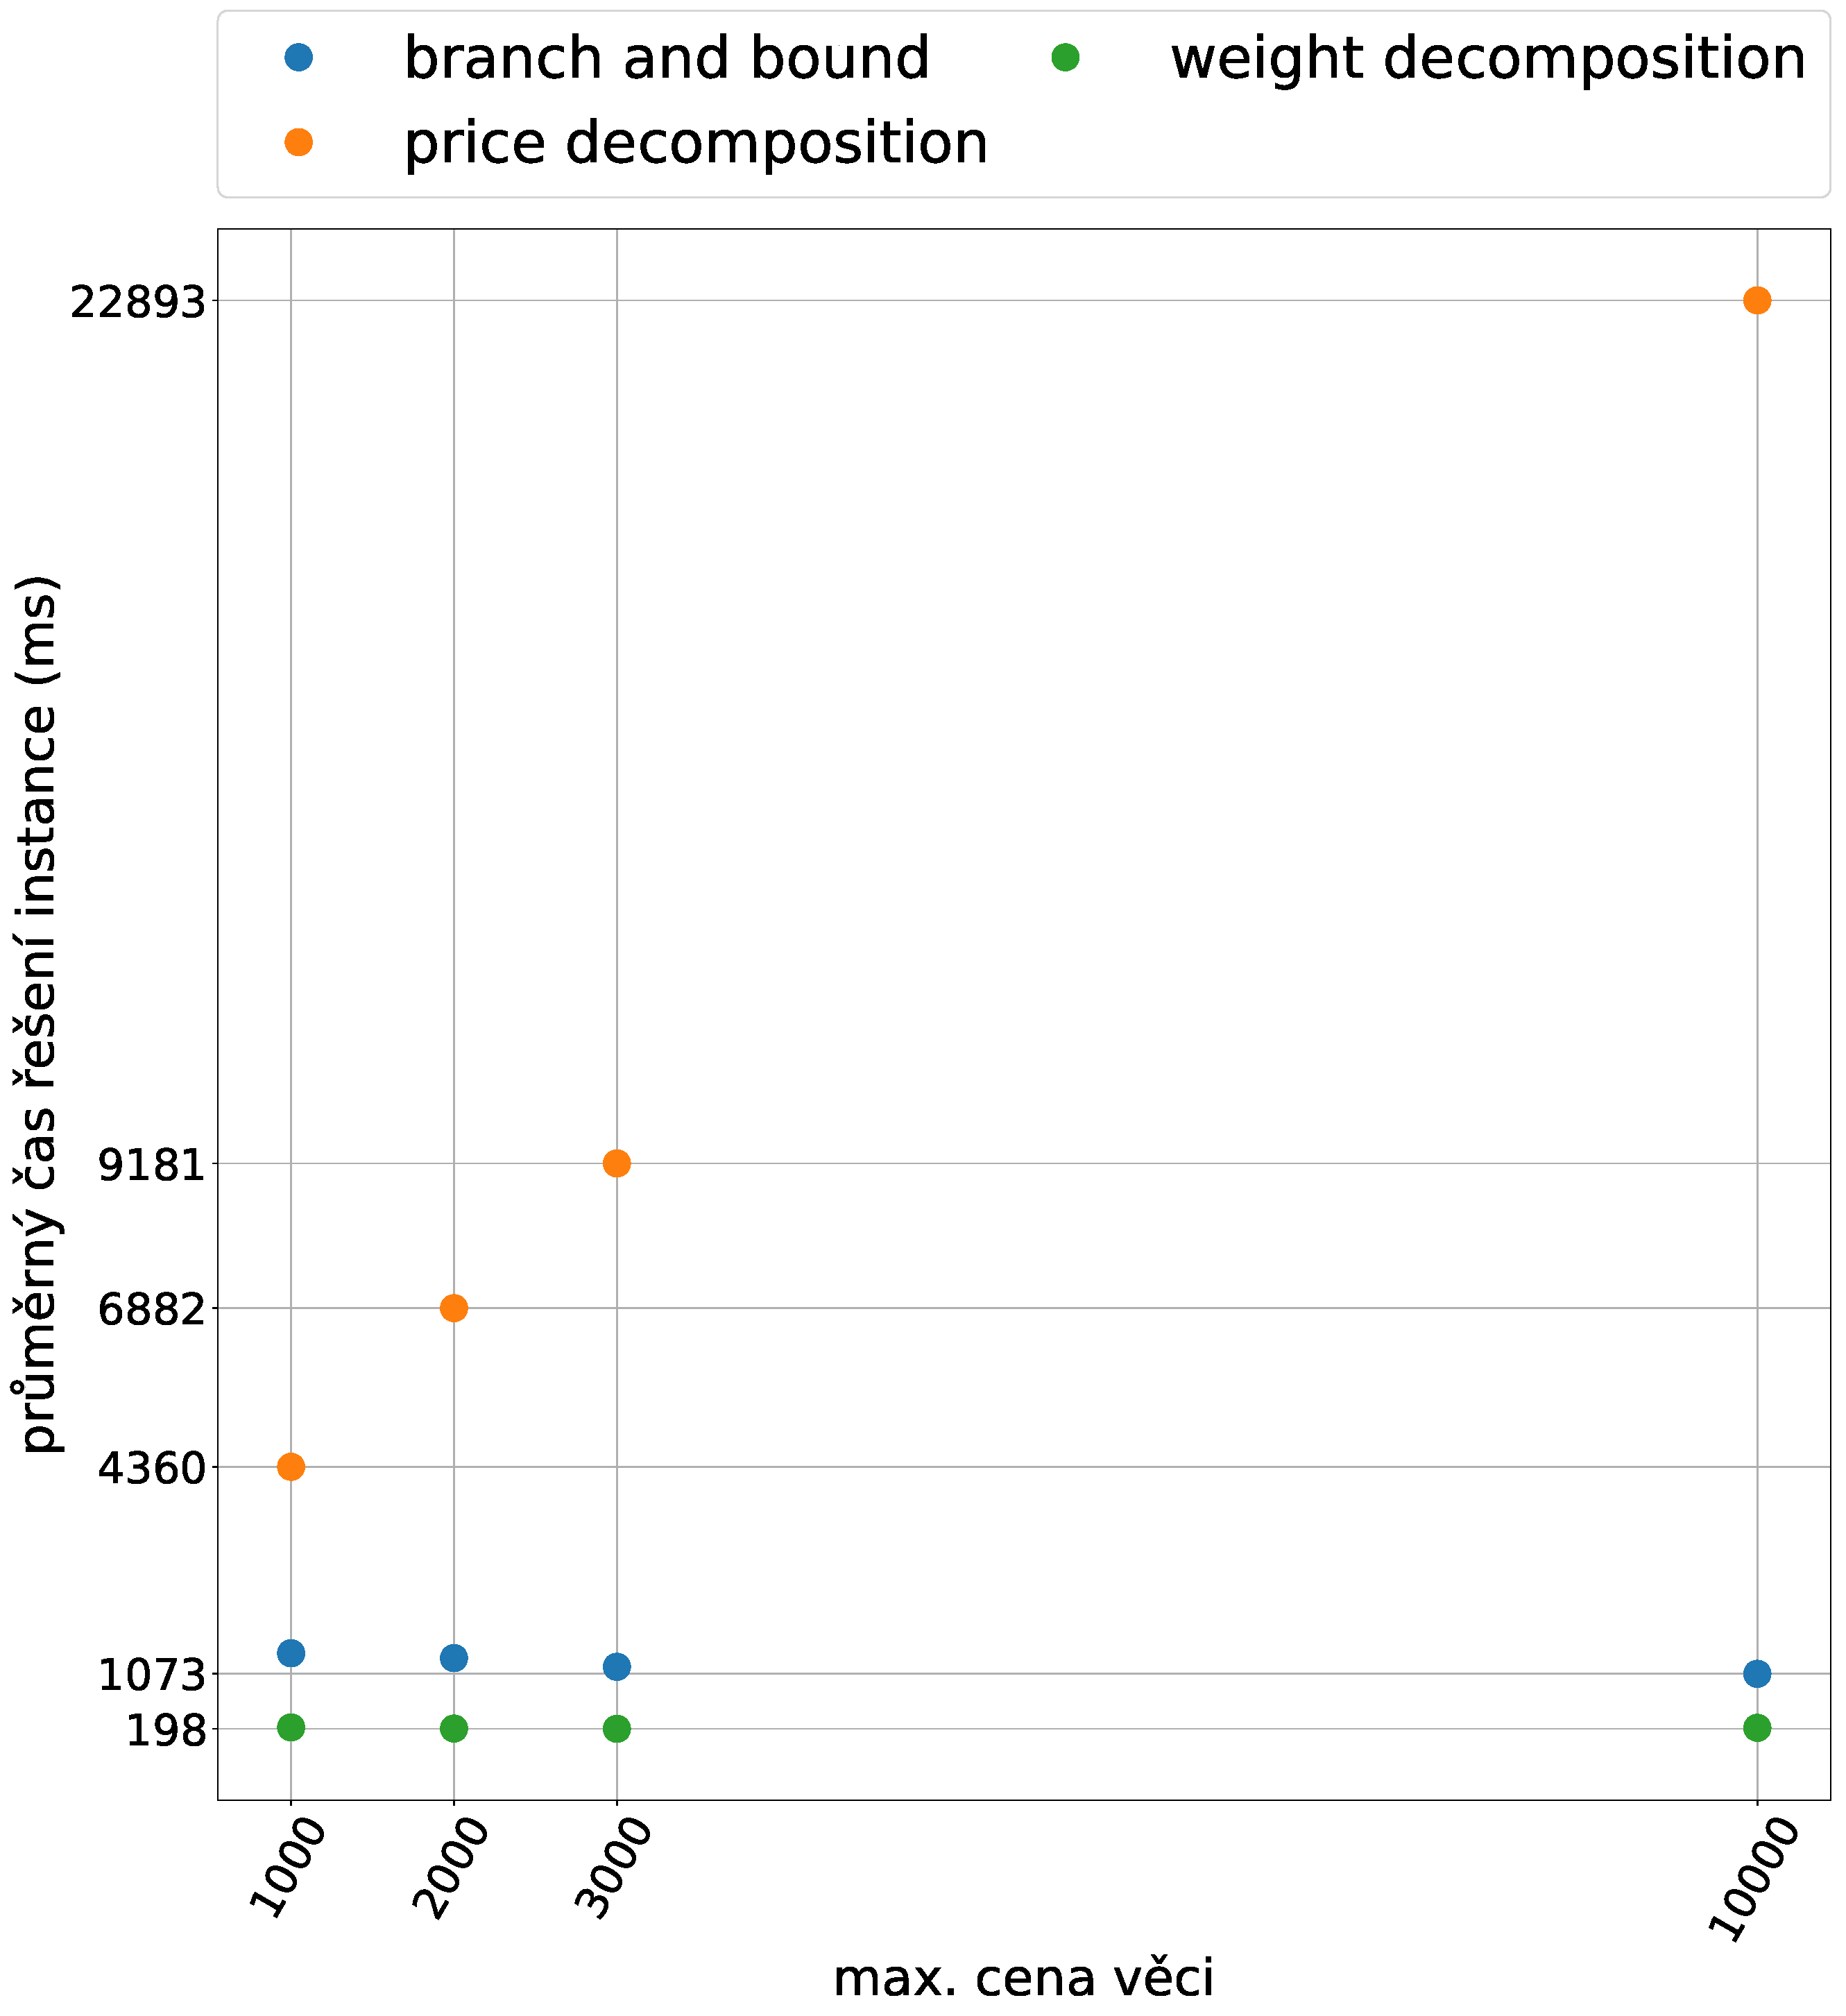
\includegraphics[width=\textwidth]{img/CE.pdf} 
    \end{minipage}
    \begin{minipage}[c]{0.49\textwidth}
        \centering 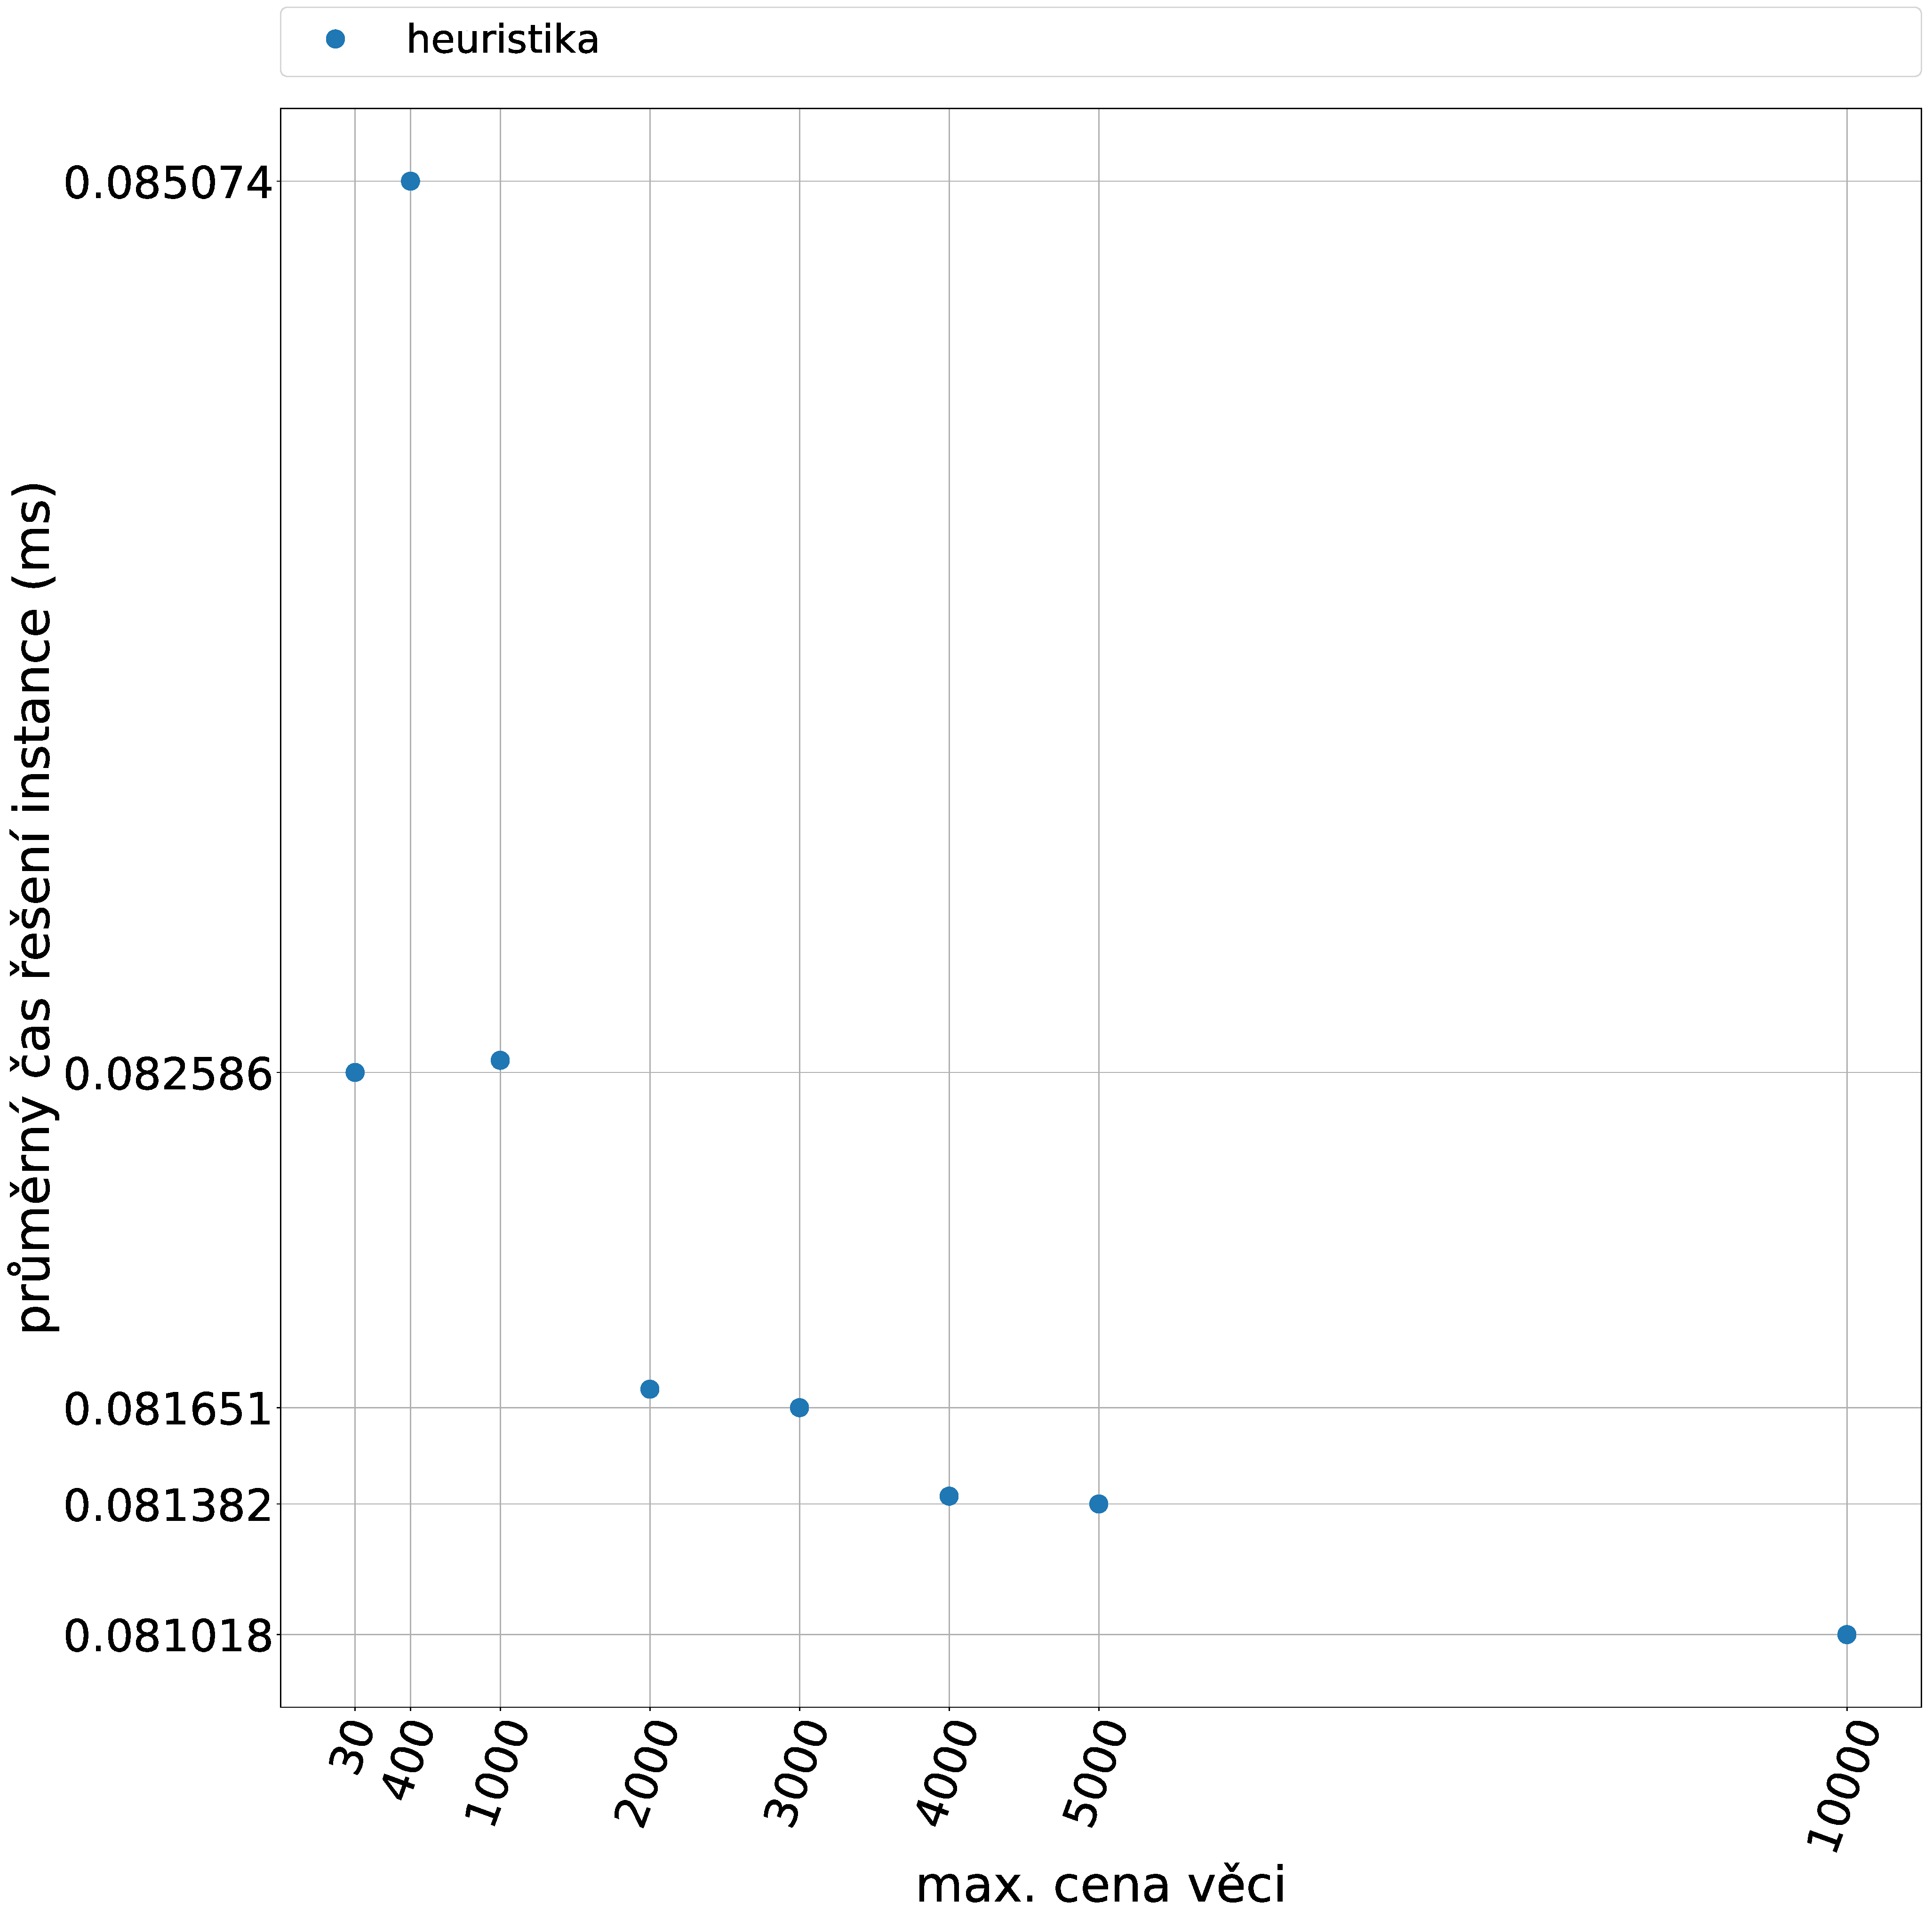
\includegraphics[width=\textwidth]{img/CH.pdf} 
    \end{minipage}
    \\
   \caption{Na grafech je vidět závislost výpočetní náročnosti na maximální ceně předmětu. Vlevo pro exaktní metody a vpravo pro heuristiku.}\label{fig:WI}
    \end{figure} 


\subsection{Závislost na maximální váze předmětů}

Závislost na maximální ceně je zobrazena na grafu \ref{fig:CI}. Je zde jasně patrné, že na tomto parametru je závislá dekompozice podle váhy, kde její čas velice rychle nárůstá. Ostatní exaktní metody nejsou závislé na maximální váze předmětu. 

Heuristika z grafu vypadá, že na maximální váhu citlivá není. Ale test nebyl prveden v tak velkém rozsahu, aby bylo možné stanovit jasný závěr.

Na grafu \ref{fig:WCEI} vlevo je zobrazena relativní chyba v závislosti na parametru maximální váhy. Z velkého rozptylu v grafu je patrné, že chyba není závislá na maximální váze. 

\begin{figure}
	\centering
    \begin{minipage}[c]{0.49\textwidth}
        \centering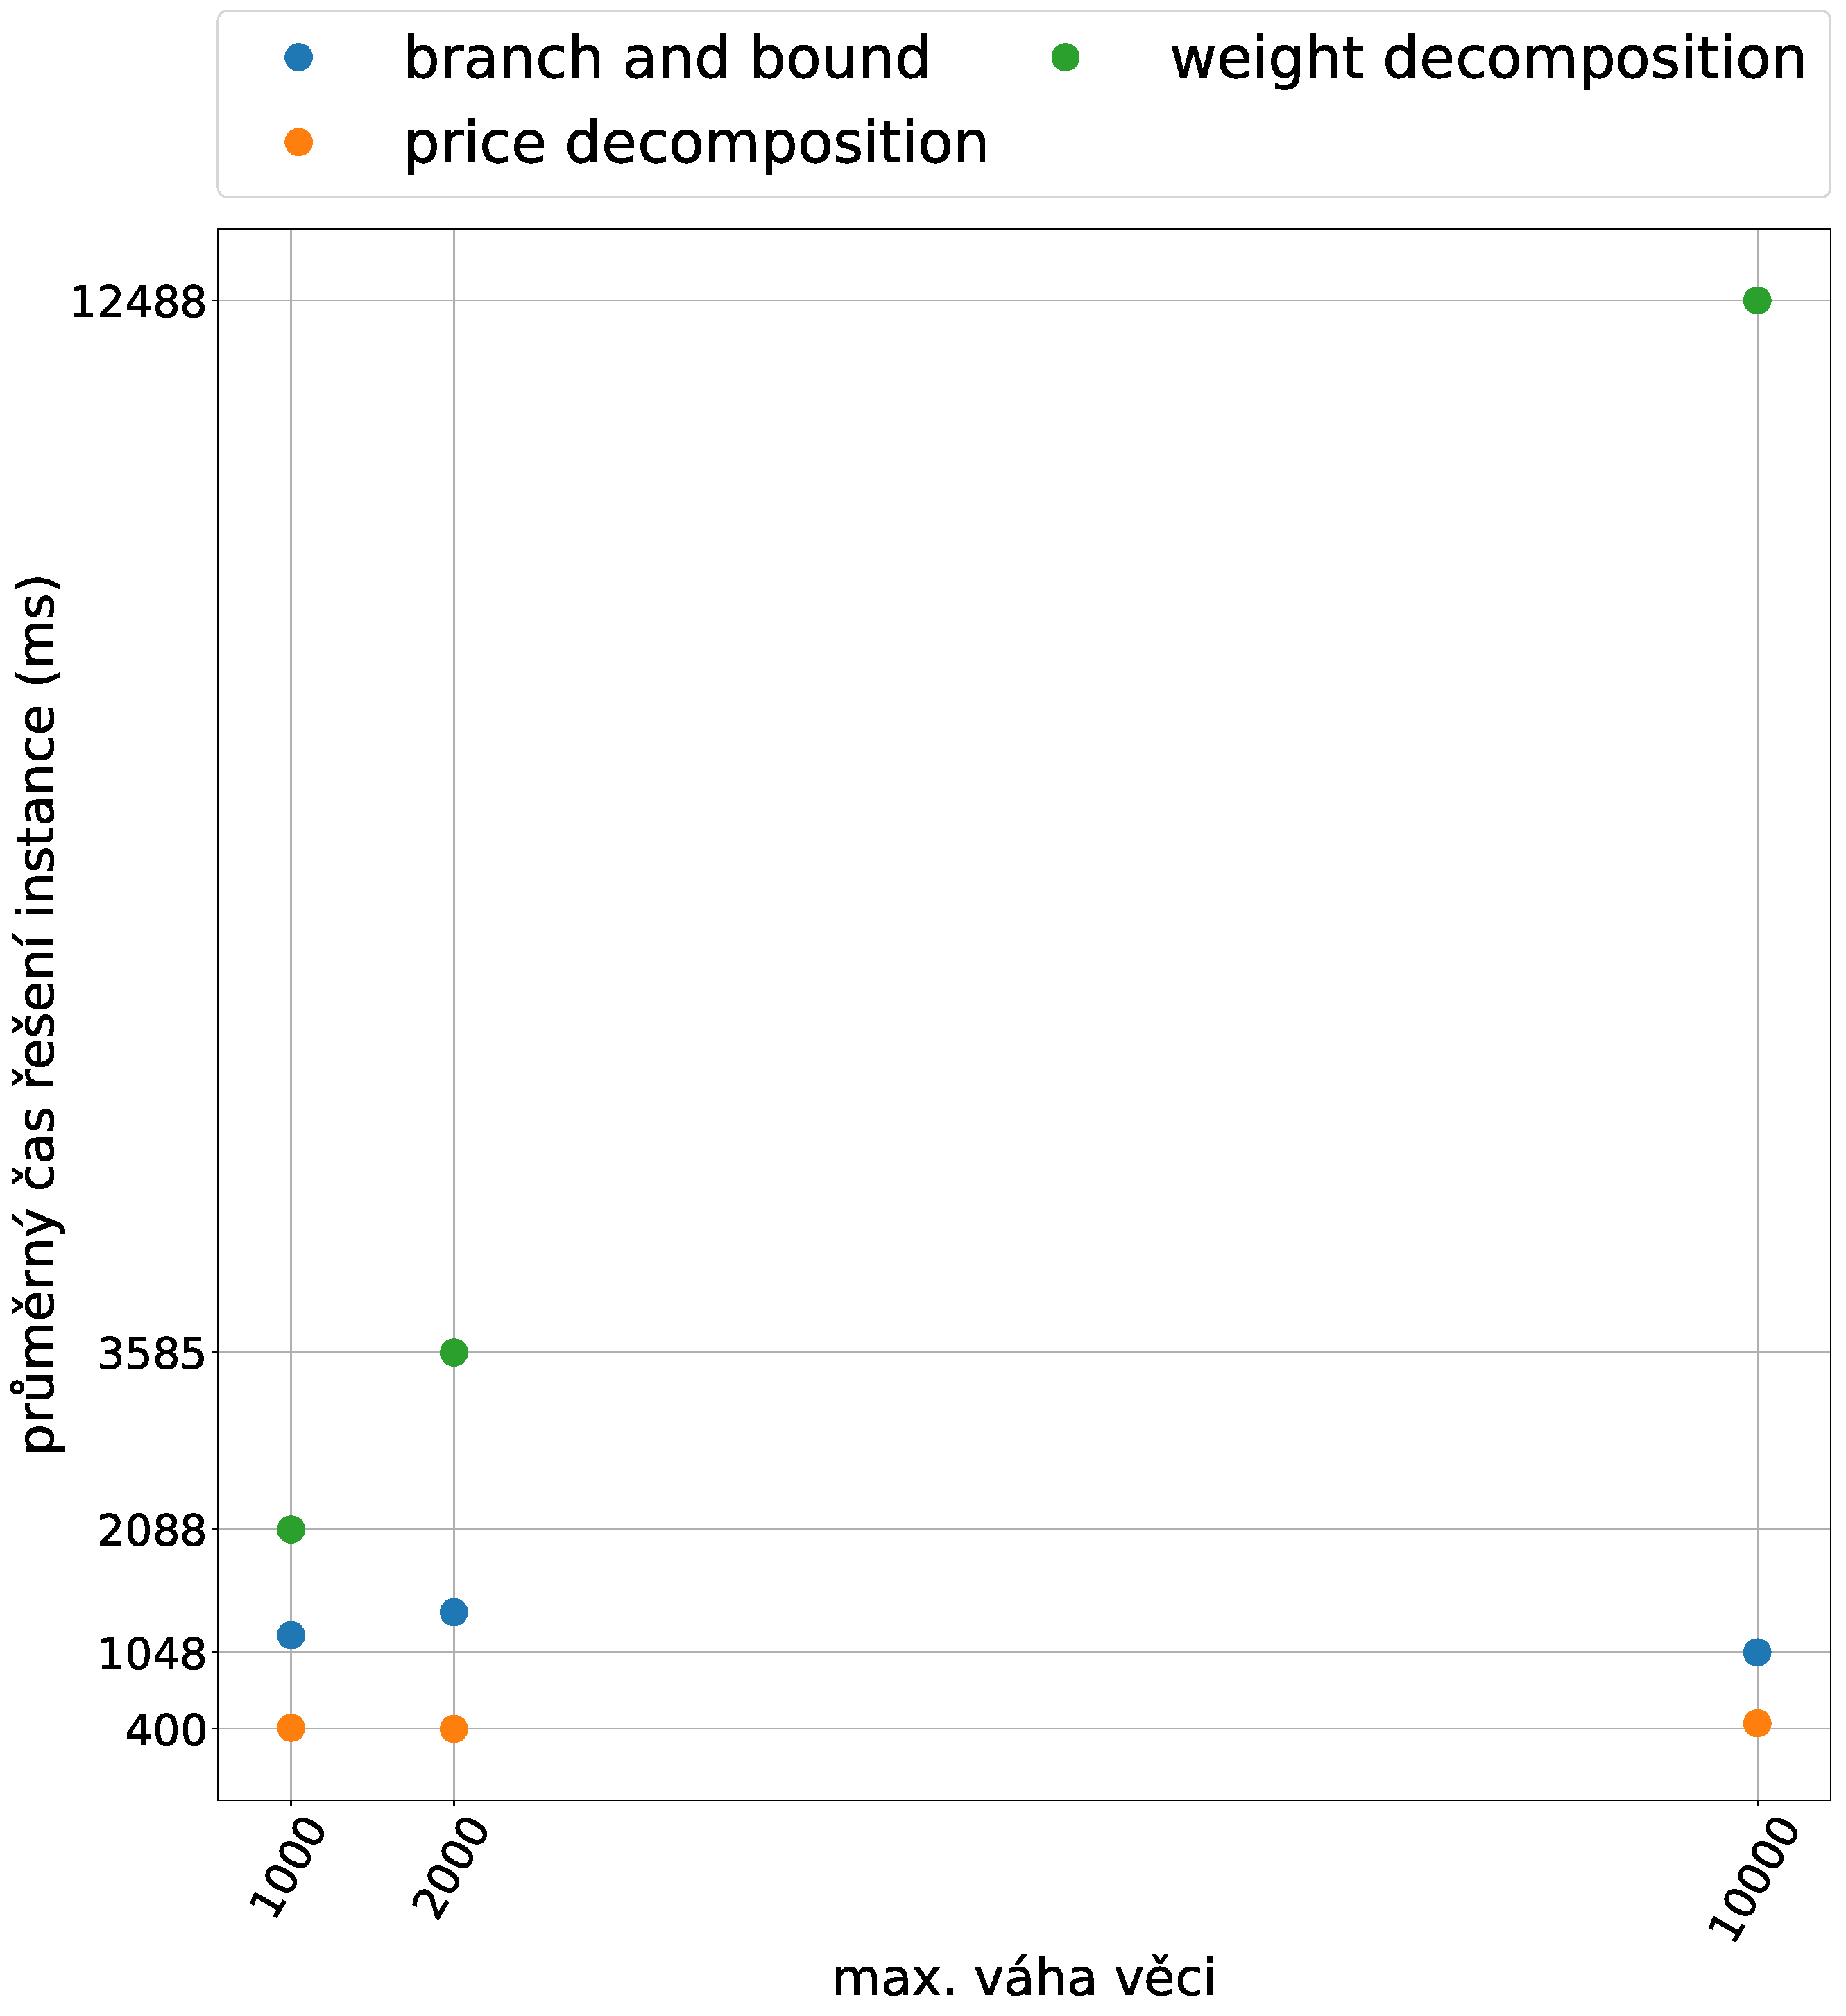
\includegraphics[width=\textwidth]{img/WE.pdf} 
    \end{minipage}
    \begin{minipage}[c]{0.49\textwidth}
        \centering 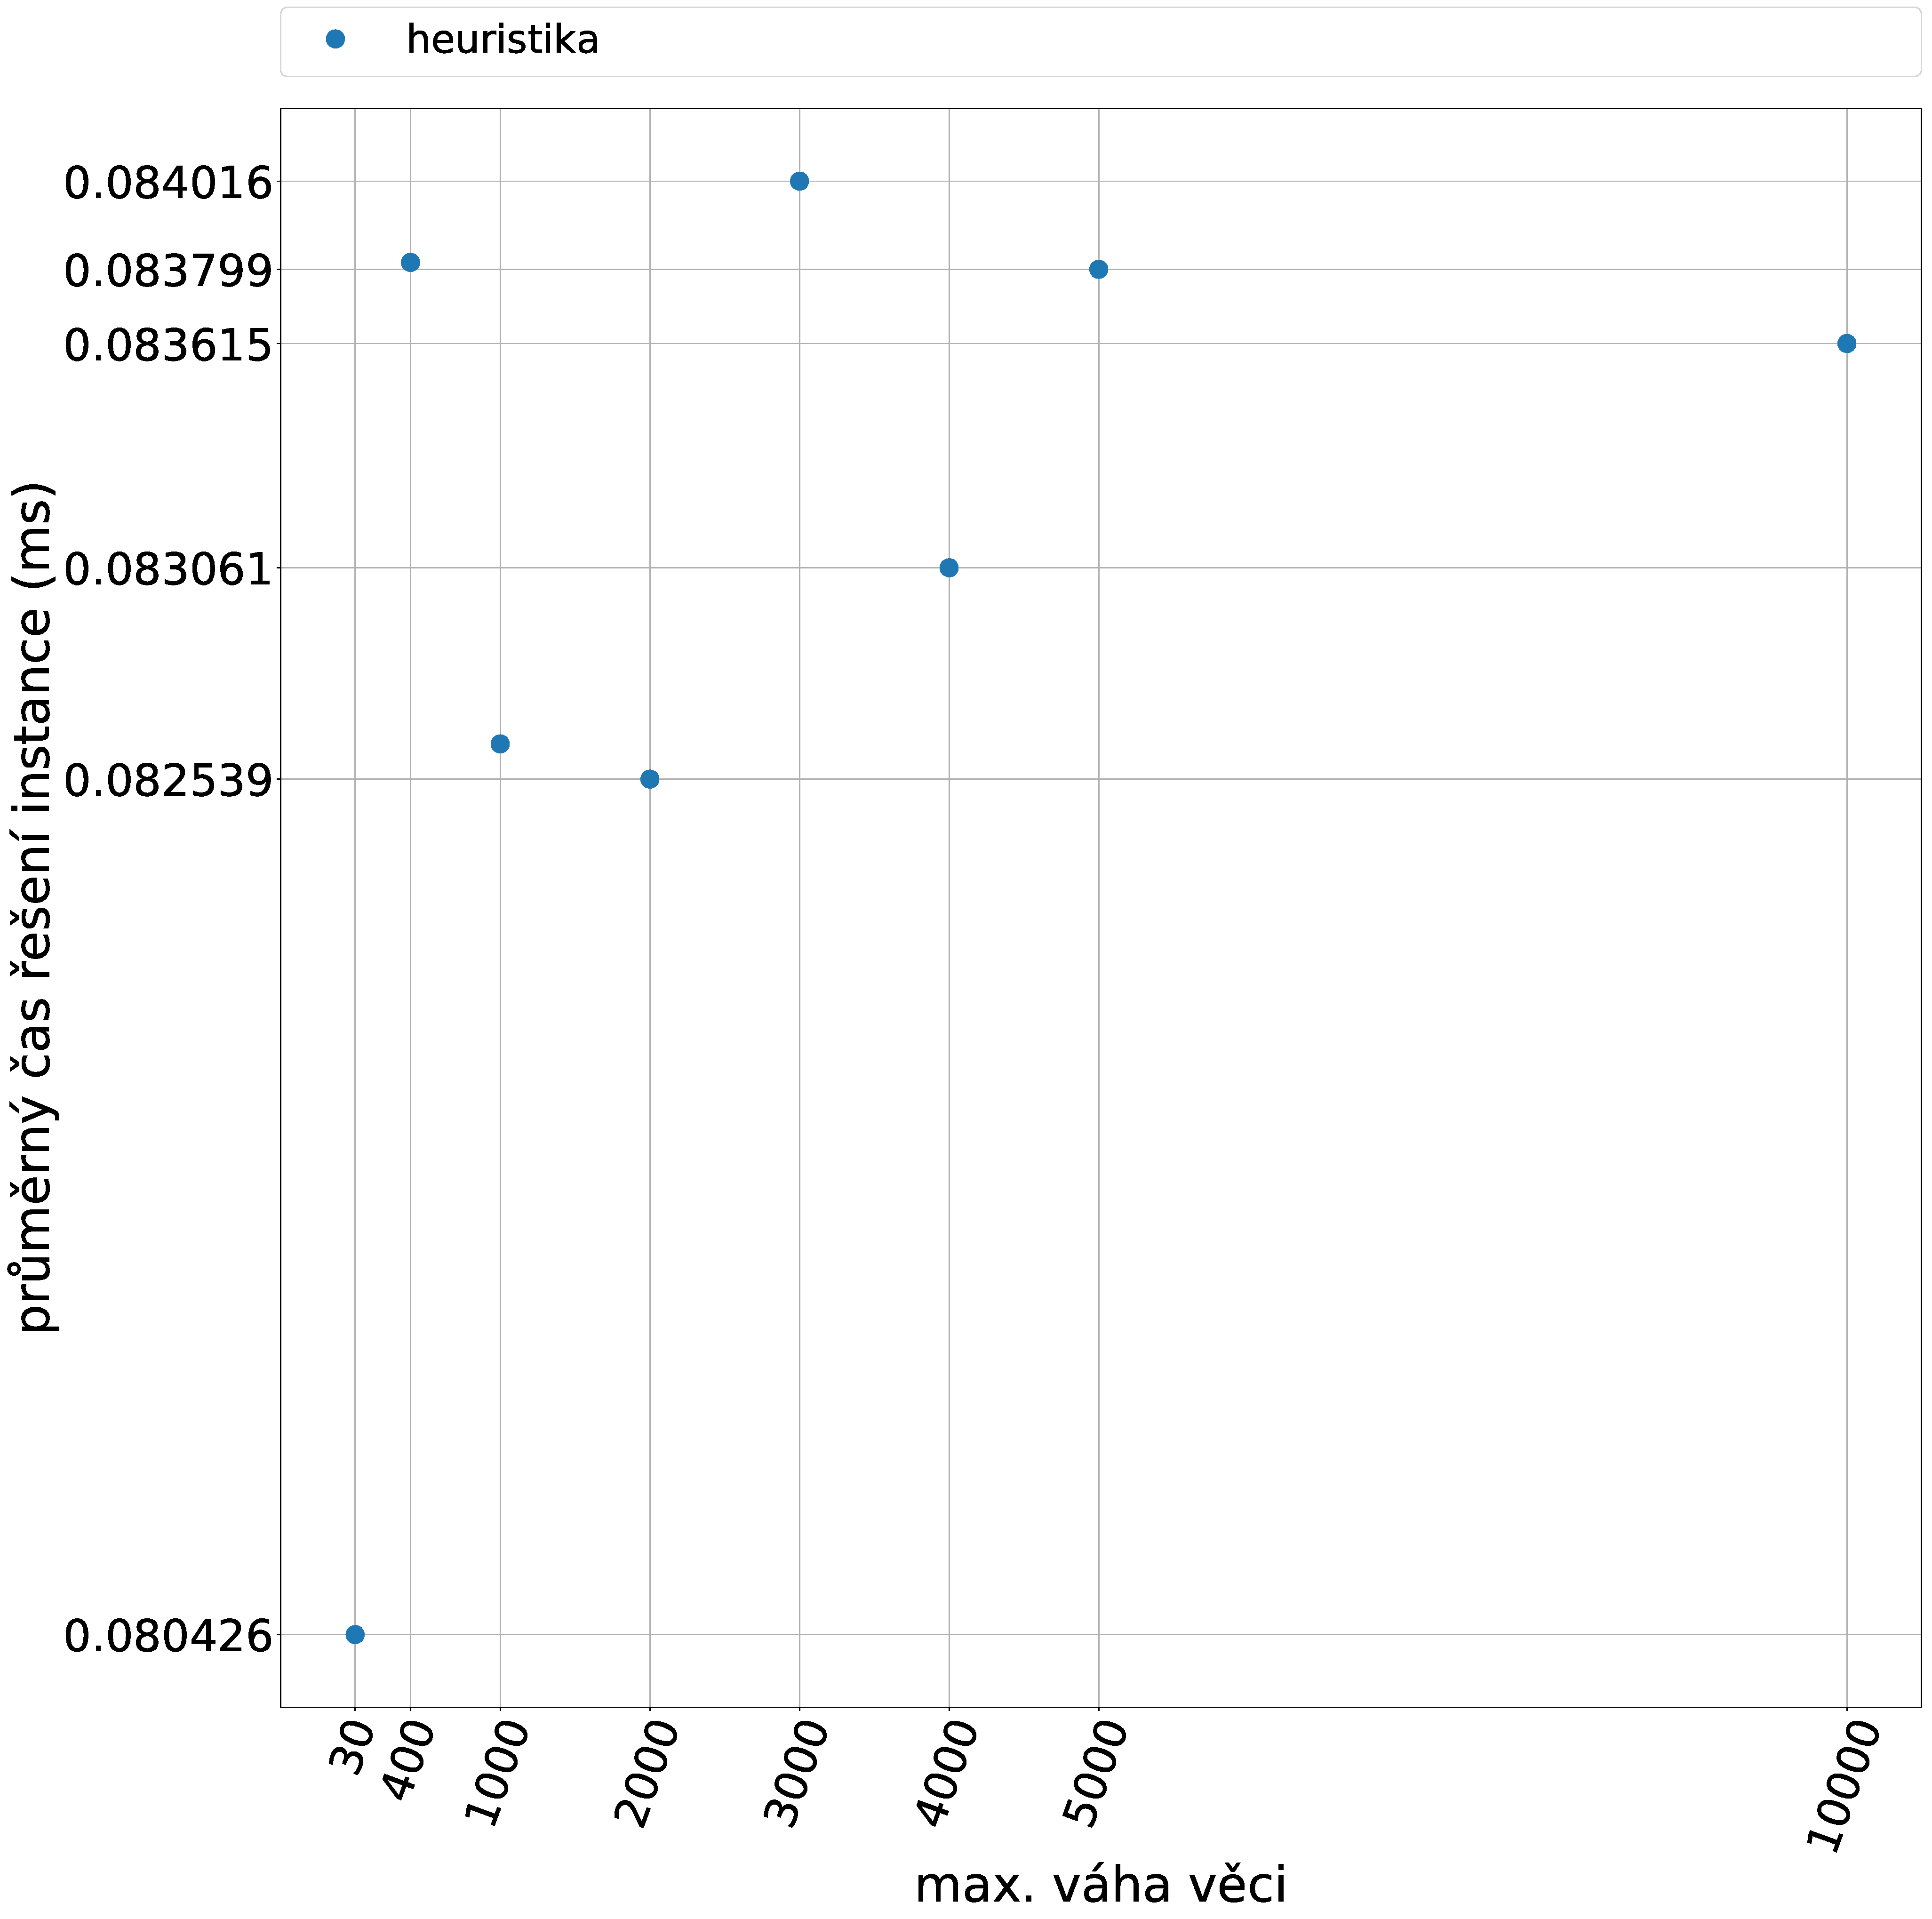
\includegraphics[width=\textwidth]{img/WH.pdf} 
    \end{minipage}
    \\
   \caption{Na grafech je vidět závislost výpočetní náročnosti na maximální váze předmětu. Vlevo pro exaktní metody a vpravo pro heuristiku.}\label{fig:CI}
    \end{figure} 
        
    
\begin{figure}
	\centering
    \begin{minipage}[c]{0.49\textwidth}
        \centering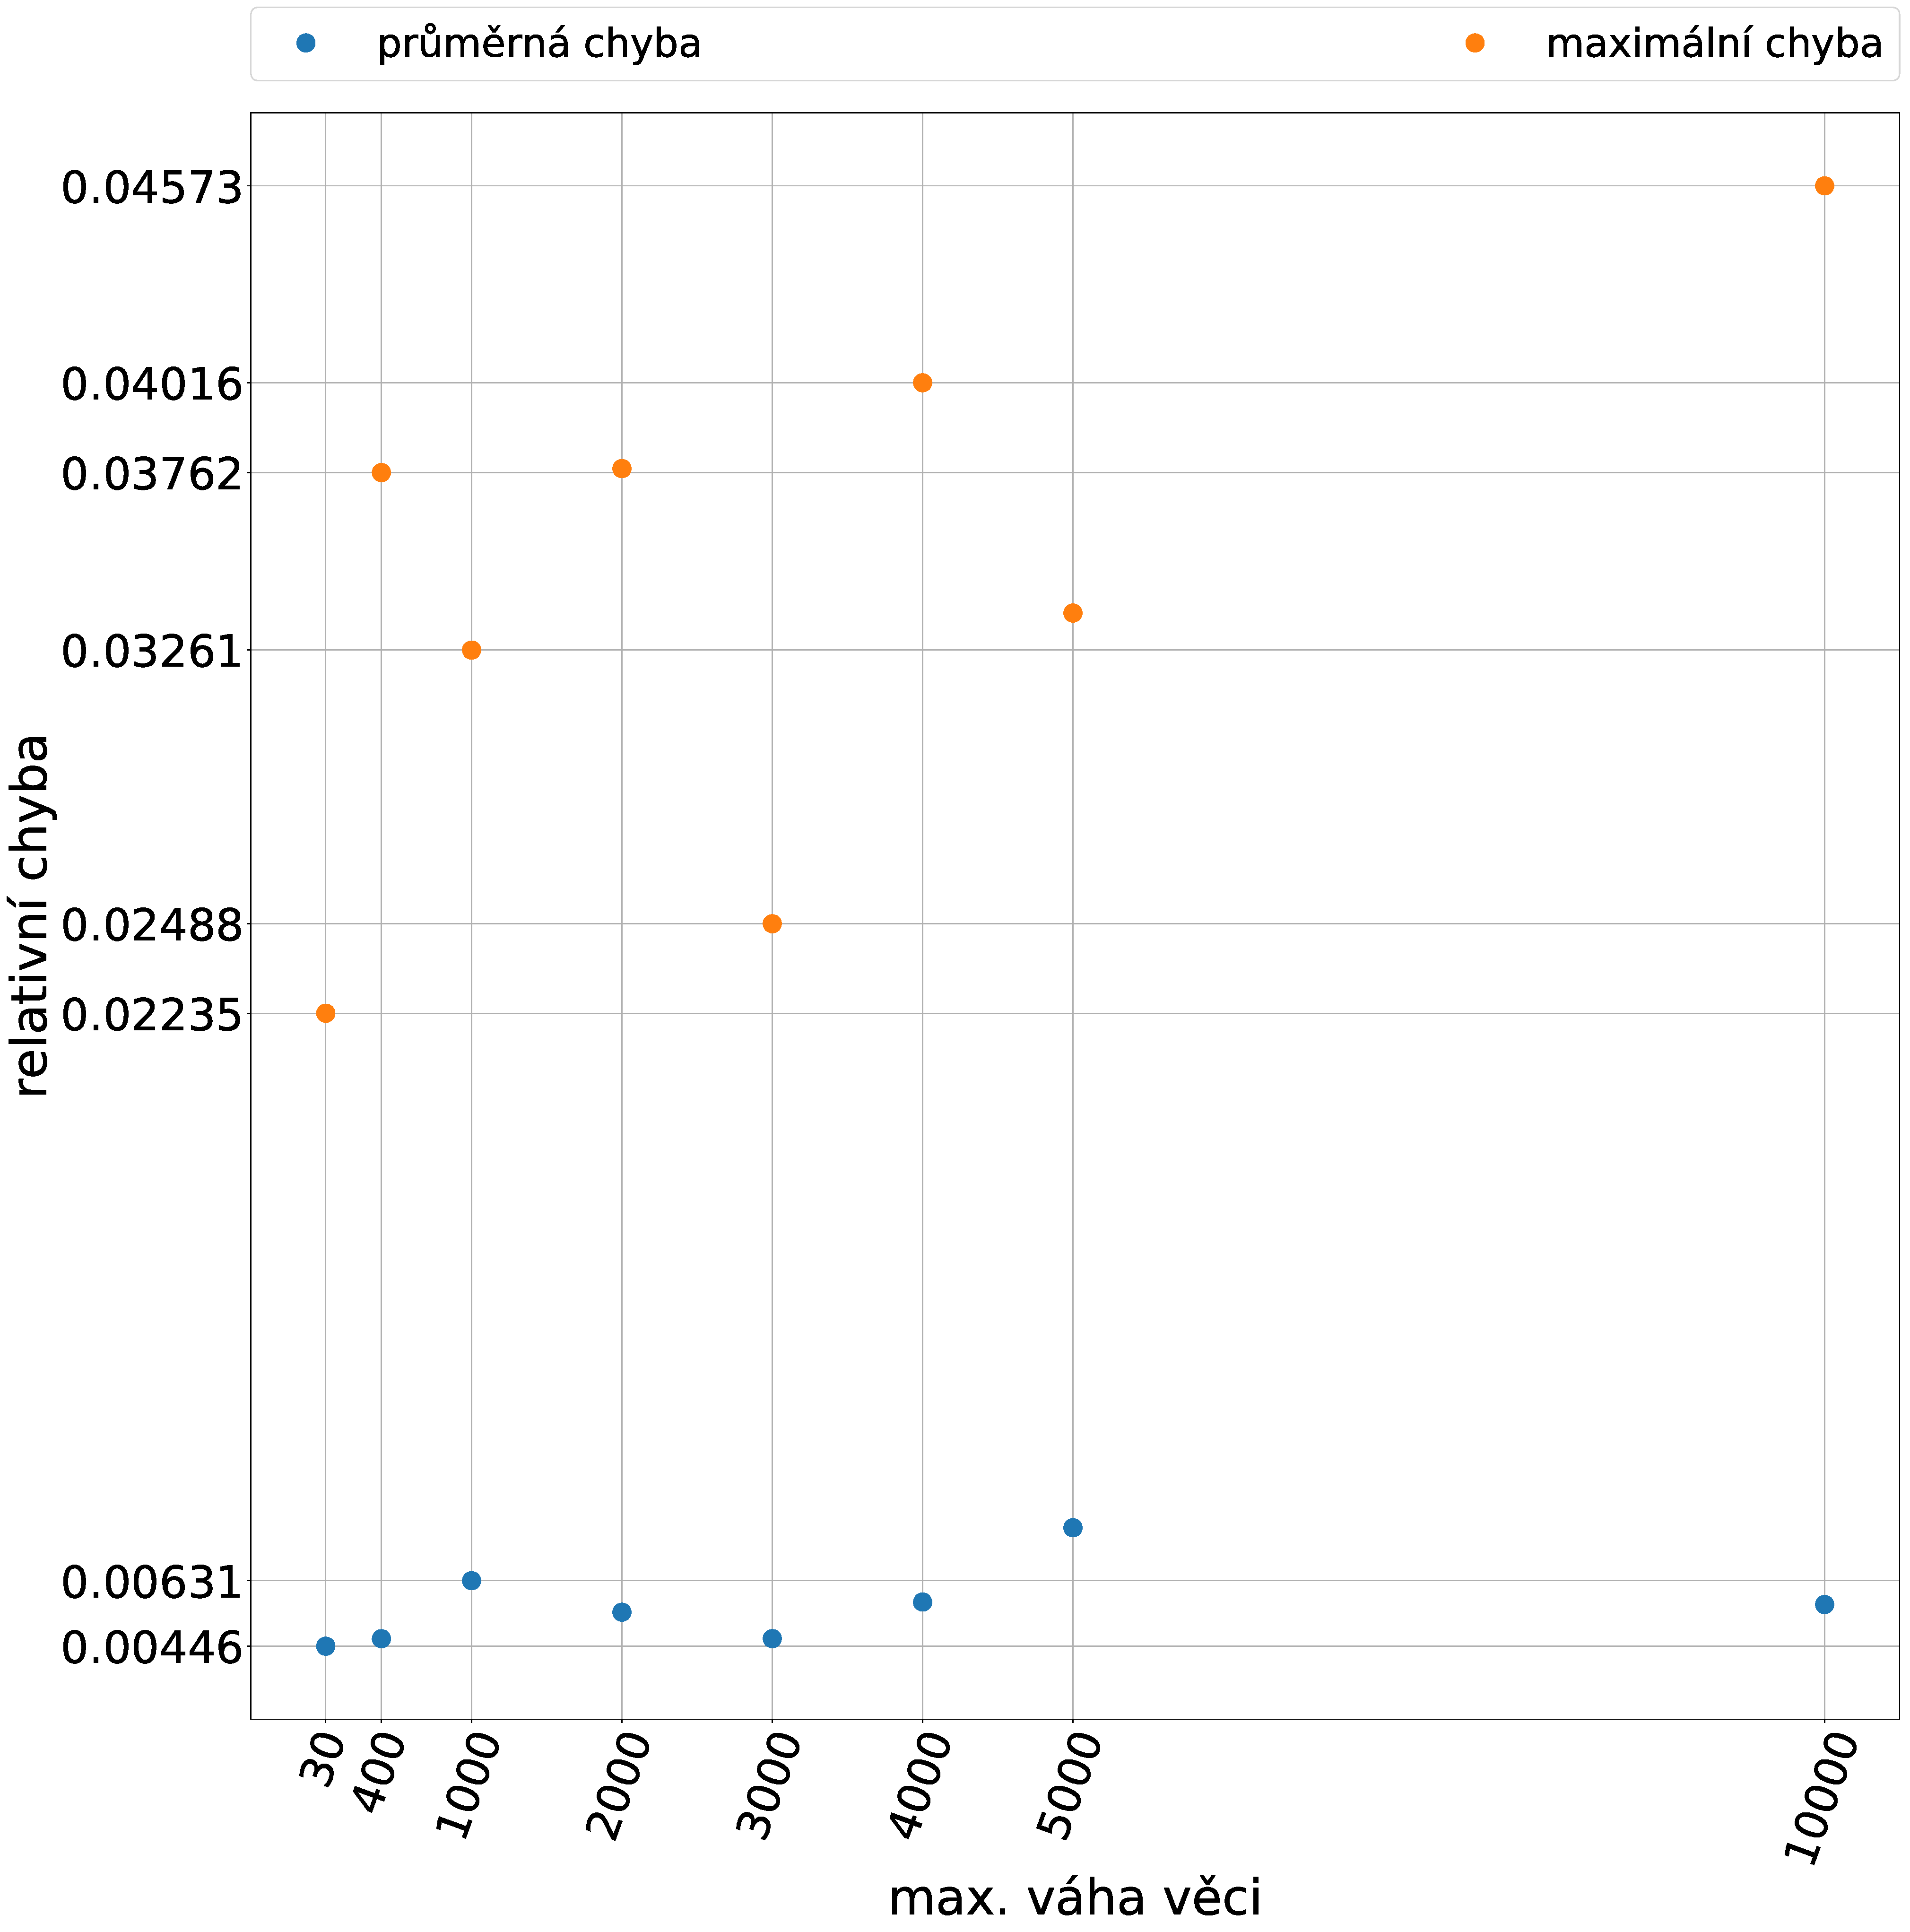
\includegraphics[width=\textwidth]{img/WHE.pdf} 
    \end{minipage}
    \begin{minipage}[c]{0.49\textwidth}
        \centering 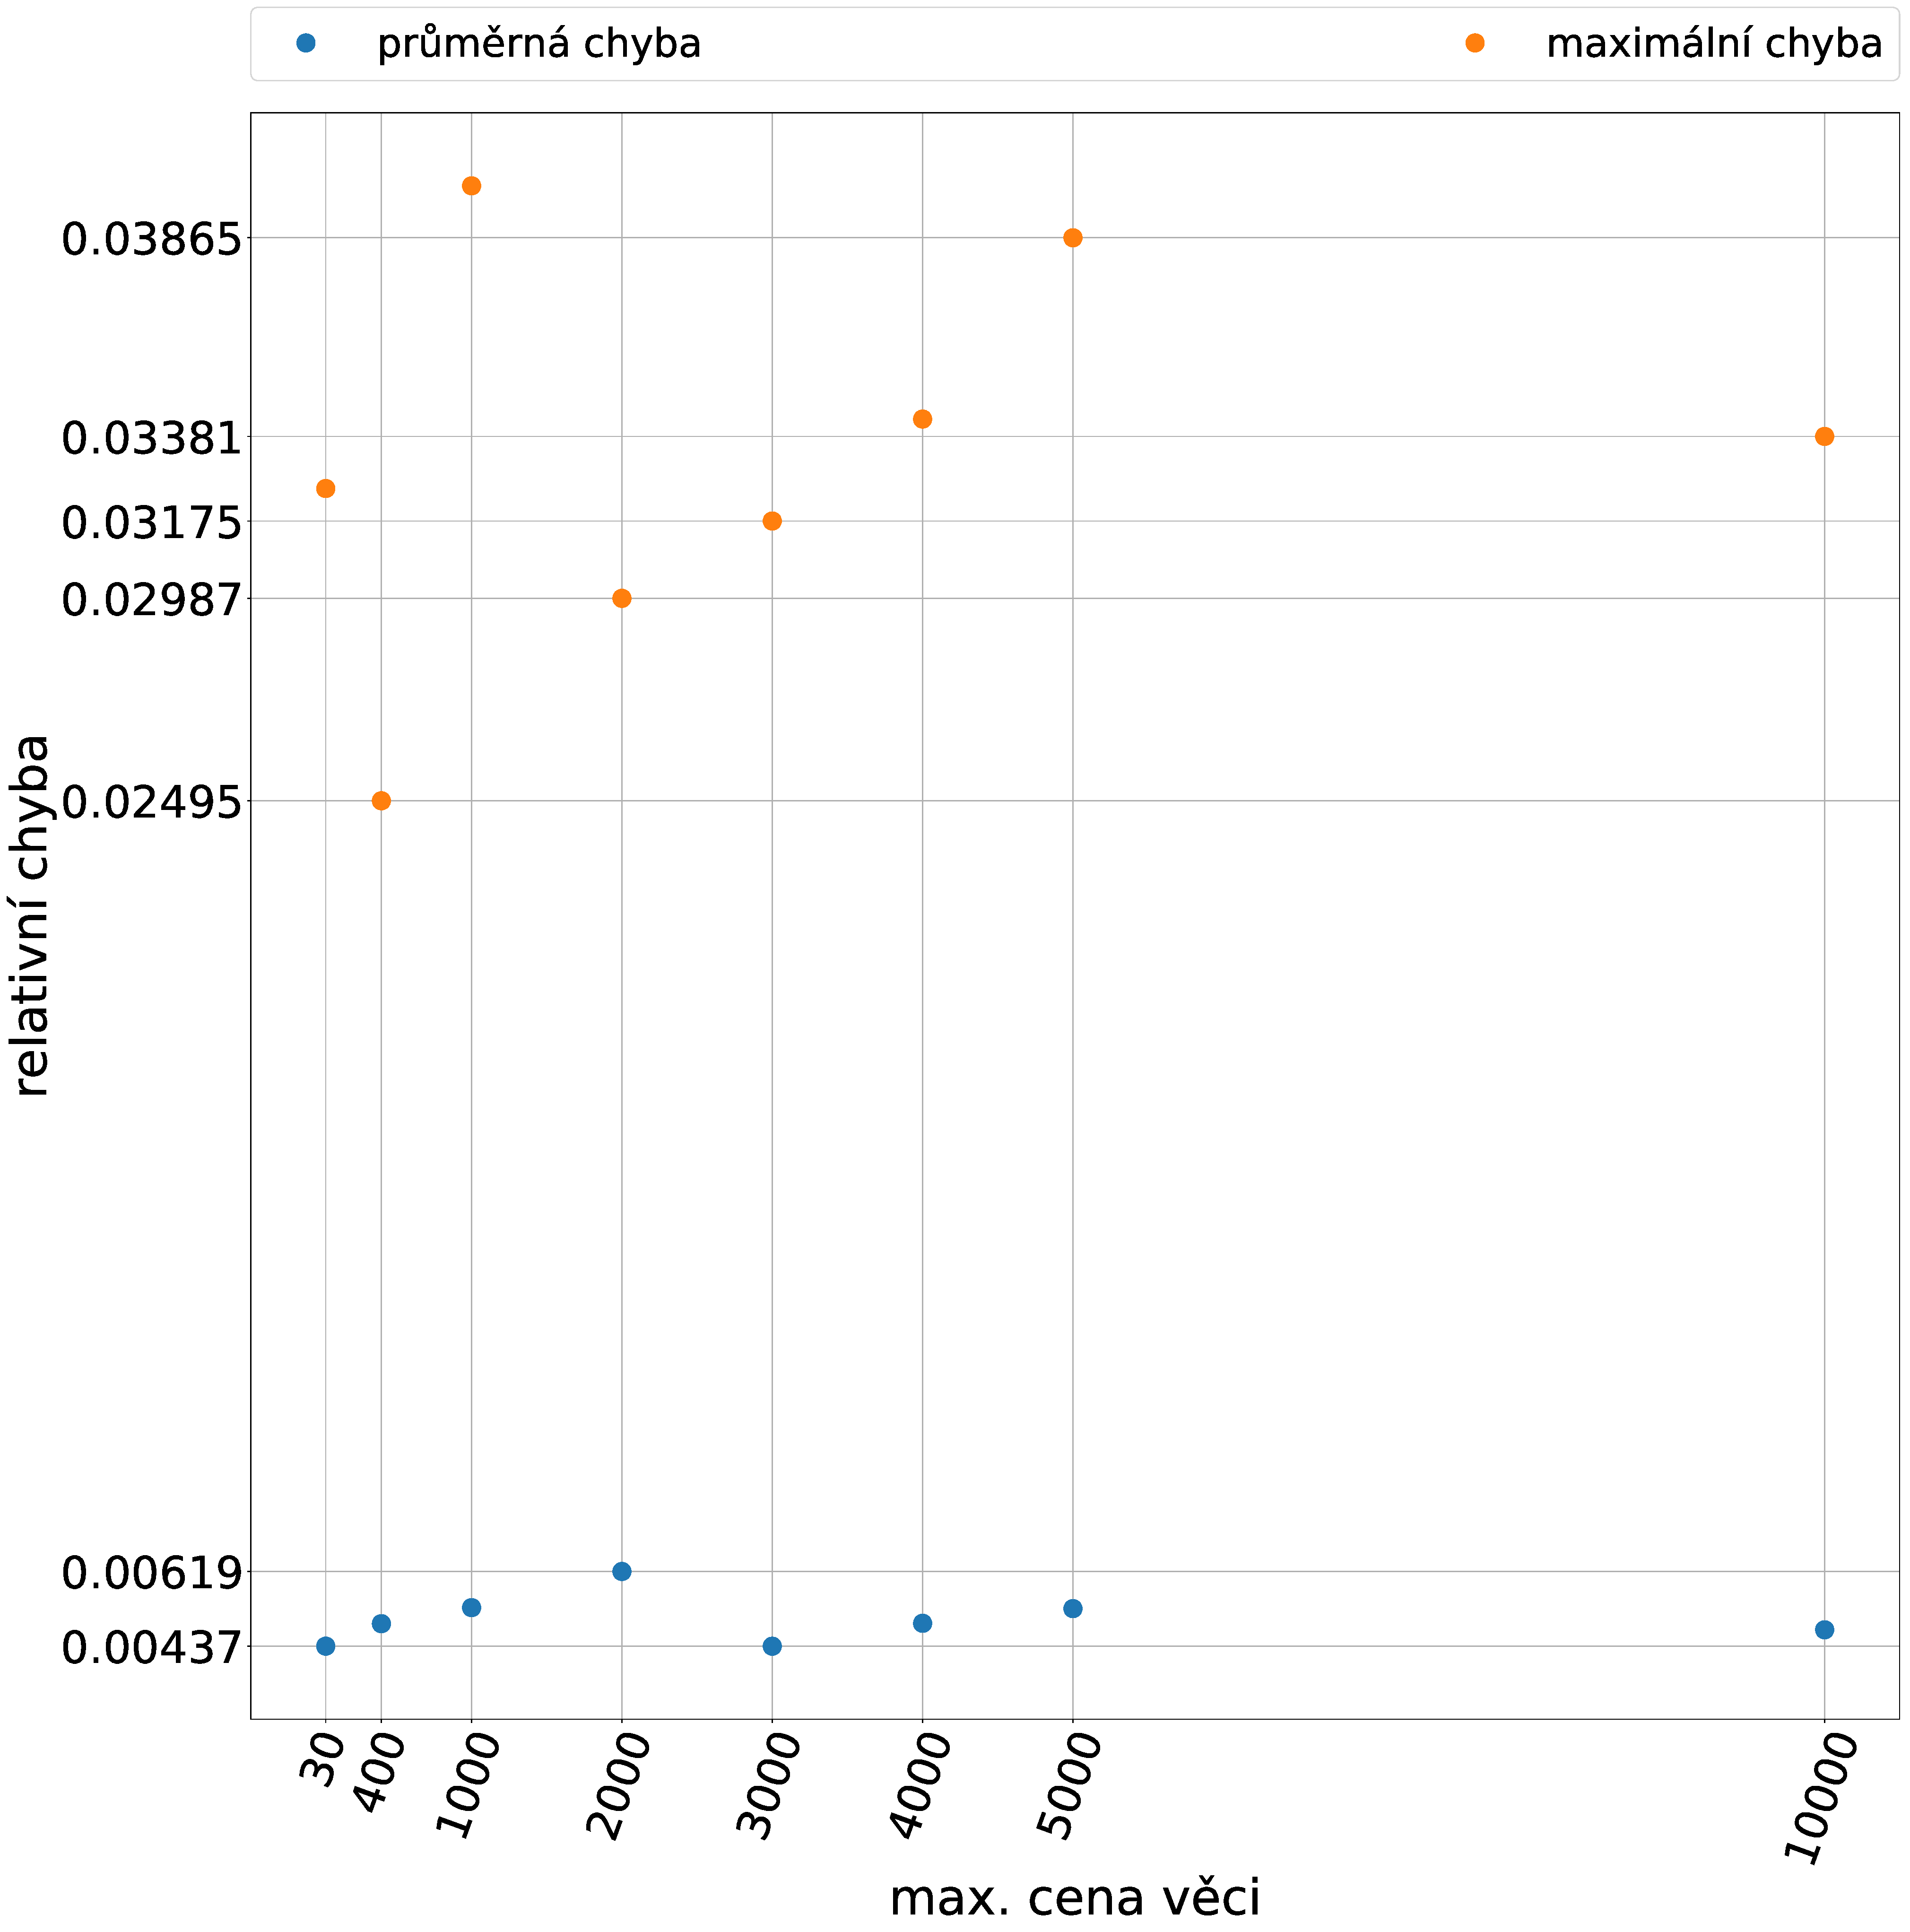
\includegraphics[width=\textwidth]{img/CHE.pdf} 
    \end{minipage}
    \\
   \caption{Na grafech je ukázána vždy průměrná a maximální chyba heuristiky v závislosti maximální váze předmětů (vlevo) a maximální ceně předmětů(vpravo). Na levém grafu pro převahu malých instancí a na převém grafu pro převahu velkých instancí.}\label{fig:WCEI}
    \end{figure} 
    
   




\section{Závěr}
Během experimentu jsem otestoval velké množství instancí s různými parametry a sledoval citlivost algoritmů na tyto parametry. Byly pozorovány časy exaktních algoritmů a u heuristiky byla také měřena relativní chyba v závislosti na změnách konkrétních parametrů instancí. 

Podle předpokladů se ukázala metoda větví a hranic citlivá na poměr sumy vah a kapacity batohu, se zvyšujícím se poměrem rostla náročnost a výpočetní složitost této metody. Až pro hodnotu 1 spadl čas na minimum, protože metoda přidá všechy předměty. Na tento poměr se také ukázala být citlivá heuristická metoda a to především co se týče relativní chyby, která klesala se snižujících se poměrem. 

V algoritmech se také projevuje nepatrně koeficient granularity, ale pouze minimálně. Na relativní chyby heuristiky vliv nemá. 

Dále se projevila závislost jednotlivých dekompozicích vždy na parametru podle kterého je prováděna. Tato znalost by nám mohla při analýze problému pomoc vybrat správný algoritmus pro minimalizaci výpočetní náročnosti. 

Velice zajímavé bylo oproti úkolu 2, že se metoda větví a hranic vykazovala větší náročnost než dynamické programování, oproti poznatku z úkolu 2 na referenčních instancí. Tento poznatek bych připsal zvolenému základnímu poměru součtu vah předmětů k nosnosti batohu. Ten činil 0.5 a tato metoda se na tento poměr ukázala velice citlivá.

Náměřené hodnoty však slouží pouze jako podpůrné argumety i přes větší množství instancí a velké množství opakování. Míra důvěry v naměřené data však souvisí na způsobu provádění experimentu a generovaných datech. 


\end{document}